% !TeX encoding = UTF-8
% !TeX spellcheck = en_US

\documentclass[
	ruledheaders=chapter,
	class=report,
	thesis={type=master, department=inf},
	accentcolor=1c,
	custommargins=true,
	marginpar=false,
	parskip=half-,
	fontsize=11pt,
]{tudapub}

\usepackage[english]{babel}

\usepackage[autostyle]{csquotes}
\usepackage{microtype}

\usepackage{enumerate}
\usepackage{enumitem}

\usepackage{biblatex}
\bibliography{thesis-literature}

\usepackage{tabularx}
\usepackage{booktabs}

\usepackage{mathtools}
\usepackage{amssymb}

\usepackage{subcaption}

\usepackage{graphicx}
\usepackage{float}
\usepackage[export]{adjustbox}
\usepackage[font=small,labelfont=bf]{caption}
\graphicspath{ {./images/} }

\newcommand{\breakable}[2][c]{%
	\begin{tabular}[#1]{@{}c@{}}#2\end{tabular}}

\counterwithout{footnote}{chapter}

\pagenumbering{roman}

\begin{document}
	\Metadata{
		title=Evaluating the Efficacy of Gaussian Padding on Website Fingerprinting Attacks,
		author=Johannes Leupold
	}
	
	\title{Evaluating the Efficacy of Gaussian Padding on Website Fingerprinting Attacks}
	\author[J. Leupold]{Johannes Leupold}
	\birthplace{Dresden}
	\reviewer{Jean-Paul Degabriele \and Vukasin Karadzic}

	\department{inf}
	\institute{IT Security}
	\group{Cryptography and Network Security}
	
	\submissiondate{01.09.2021}
	\examdate{20.09.2021}
	
	% Hinweis zur Lizenz:
	% TUDa-CI verwendet momentan die Lizenz CC BY-NC-ND 2.0 DE als Voreinstellung.
	% Die TU Darmstadt hat jedoch die Empfehlung von dieser auf die liberalere
	% CC BY 4.0 geändert. Diese erlaubt eine Verwendung bearbeiteter Versionen und
	% die kommerzielle Nutzung.
	% TUDa-CI wird im nächsten größeren Release ebenfalls diese Anpassung vornehmen.
	% Aus diesem Grund wird empfohlen die Lizenz manuell auszuwählen.
	% \tuprints{urn=1234,printid=12345,doi=10.25534/tuprints-1234,license=cc-by-4.0}
	% To see furhter information on the license option in English, remove the license= key and pay attention to the warning & help message.
	
	% \dedication{Für alle, die \TeX{} nutzen.}
	
	\maketitle
	
	\affidavit[digital]% oder \affidavit[digital] falls eine rein digitale Abgabe vorgesehen ist.

	\begin{abstract}[english]
		Website Fingerprinting (WF) attacks pose a serious threat to internet users' privacy, being effective against popular anonymization services such as Tor. For this reason, various countermeasures against WF have been considered. A major class of such countermeasures are padding schemes, out of which randomized schemes have previously shown to achieve good results with a high bandwidth efficiency. Up to now, only uniformly distributed padding lengths have been examined. This thesis contributes a comprehensive study of padding using the Gaussian distribution, evaluating it against a selection of WF attacks and estimating a formal bound on the efficacy of this scheme. It shows that the Gaussian distribution achieves better results against certain attacks than the uniform distribution. However, it is also revealed that Gaussian padding is insufficient to defend against recent WF attacks. In particular, the results point out that simple randomized padding schemes are unlikely to reliably disguise coarse-grained properties of websites, and therefore aren't sufficient on their own to defend against attacks using those properties.
	\end{abstract}
	
	\tableofcontents
	
	\chapter{Introduction}
	\label{introduction}
	\IMRADlabel{introduction}
	\pagenumbering{arabic}

	Preserving privacy while surfing the internet has become an increasingly sensitive topic over the last two decades. The web keeps extending into every day life, while at the same time, the emergence of actors interested in gaining insights into the browsing behavior of individuals raises concerns about the loss of privacy. On the one hand, there are large internet companies trying to gain information about a user's interests for the sake of profit. While this may be undesirable and possibly reprehensible from a data protection standpoint, the certainly more concerning development is the presence of nation-state adversaries that are collecting data on citizens for mass surveillance, state censorship or even the criminal prosecution of dissidents. For this reason, SSH or VPN tunnels and anonymization services such as Tor\footnote{\url{https://www.torproject.org/}} have experienced a steady climb in popularity, especially after relevant events, such as the Snowden revelations in 2013 \cite{TorHistory}.
	
	Unfortunately, Website Fingerprinting (WF) research has shown that it is not only possible to identify which websites a user has visited from the raw network packet sizes, but to do so with high accuracy and robustness (cf. \cite{Liberatore2006,Herrmann2009,Panchenko2011,Dyer2012,Wang2014,Panchenko2016,Hayes2016,Sirinam2018,Wang2021}). This fact has led to the development of various countermeasures (cf. \cite{Wright2009,Dyer2012,Cai2014,Cai2014a,Juarez2016,Luo2021}) that try to disguise the identifying characteristics of a website in the packet sizes. In particular, those defenses may change packet sizes or timing in an attempt to make it harder to distinguish individual websites or to make one website look like another. A major class of such defenses are padding schemes that increase packet sizes after some fixed algorithm. Padding sizes can be chosen deterministically or randomized, while the latter have shown to achieve better results at a higher bandwidth efficiency \cite{Dyer2012}. However, up to now only the uniform distribution has been considered to select padding sizes.
	
	In this thesis, the rounded truncated Gaussian distribution is evaluated for padding selection in the context of WF attacks. This padding distribution has already been proven effective in hiding the length of encrypted messages while also outperforming the uniform distribution significantly \cite{Degabriele2021}. Because of that, this work aims to determine whether this advantage transfers to the field of website fingerprinting. Furthermore, one goal is to draw general conclusions about the efficacy of Gaussian and other randomized padding schemes against different types of WF attacks. Building on that, a general statement about the suitability of such schemes for current and future attacks is derived.
	
	%During evaluation it shows that this advantage transfers to the field of website fingerprinting when considering attacks that use the individual packet sizes directly, whereas for attacks that use coarser-grained features Gaussian padding doesn't perform better, sometimes even worse, than uniform padding. Furthermore, the results point out that randomized padding schemes can't be considered a sufficient choice for defending against modern WF attacks.
	
	\paragraph{Source Code} The WF evaluation framework written in the course of this work is made available on Github\footnote{\url{https://github.com/Traderjoe95/website-fingerprinting}}. 

	\chapter{Background Material}
	\label{fingerprinting}

	\section{Theoretical Setting}
	\label{theoretical}
	
	Website Fingerprinting (WF) is a field of study focusing on data leaked from anonymization 
	techniques and whether it is still sufficient to conclude which websites the user visited.
	Furthermore, a goal of Website Fingerprinting study is the evaluation of various countermeasures
	that limit the leaked data and thus thwart attempts to uncover the websites a certain user was
	visiting.
	
	\subsection{Threat Model}
	\label{theoretical:threat_model}
	
	The Website Fingerprinting adversary is assumed to have access to the encrypted network traffic of the victim. However, he is not able to decrypt the traffic, or parts of it, so he can only draw conclusions based on metadata of the encrypted packets. Furthermore, he may not interfere with the traffic, such as insert or suppress packets from or to the victim. Such an adversary is called \textit{passive} (as he can't actively interfere with the system) and \textit{local} (as he can only observe local information, i.e. network packets on the victim's machine). In particular, the adversary observes 
	
	\begin{itemize}
		\item packet length (full packet size in bytes),
		\item direction (whether the packet goes from Client $\to$ Server, or vice versa), and
		\item timing (amount of time between the first packet and the current packet).
	\end{itemize}

	This information also gives way to various derived measures, such as overall bandwidth consumed, overall time, or burst\footnote{A \textit{burst} is a contiguous sequence of packets going in the same direction} length/size.
	
	Before the adversary begins with the attack, he can create a database of websites the victim may visit and collect so-called \textit{packet traces} for the websites. A packet trace is a sequence $\mathcal{T} = \langle p_1,p_2,...,p_n\rangle$ of tuples $p_i = (t_i, l_i, d_i) \in \mathbb{N} \times \{52, \ldots, MTU\} \times \{\uparrow, \downarrow\}, i = 1,\ldots,n$, where $t_i$, $l_i$ and $d_i$ denote the time, length and direction for a single observed packet, respectively. The packet length can never be smaller than 52 bytes, as that is the size of the smallest possible TCP/IP packet, the ACK packet. The maximum packet size $MTU$ (also called \textit{Maximum Transmission Unit}) is dependent on the used network technologies. For Ethernet, the MTU is 1500 bytes, while for WiFi (IEEE 802.11) it is 2312 bytes. Note that the adversary is assumed to collect his database of website traces under the same technical preconditions (network technologies) that his victim uses to access them. When carrying out the attack, the adversary observes packet traces for particular page loads of the victim. He may then use any algorithm and his prepared database to try and deduce which websites out of the pre-selected set the victim visited. When a WF countermeasure is in place, the adversary is assumed to be aware of it such that he can collect his trace database under the same countermeasure.
	
	WF threats may be considered either in the Closed World or the Open world scenario. In the Closed World, the goal of the adversary is to identify the websites a victim visited from a fixed set of websites known in advance, while in the Open World scenario, the adversary defines a set of monitored web pages and intends to identify whether the victim visited a website from that set.
	
	
	\subsection{Attacks}
	\label{theoretical:attacks}
	
	To successfully make conclusions on the websites a victim visited, the attacker needs to classify the packet traces he observed to be an instance of one of the websites in his database. He may achieve this by randomly guessing the instance's class, but this naive method can't be expected to yield good results for higher numbers of websites. Therefore, the adversary may employ a Machine Learning technique, consisting of a feature extraction\footnote{\textit{Feature Extraction} refers to transforming a certain observation into a number of (mostly numerical) attributes, called \textit{features}} and a classification algorithm. A classification algorithm is trained using a number of examples from all classes including the class labels (the \textit{training set}). In the following, an overview of common classification algorithms is given.
	
	\subsubsection{Nearest Neighbors}
	\label{ml:nn}
	
	The Nearest Neighbors classifier (also called NN) is a simple algorithm that assigns to each instance the class of its nearest neighbor according to some distance metric. It may be extended to $k$-Nearest-Neighbors ($k$-NN) by considering the nearest $k$ neighbors and taking the majority vote of their classes. One may also apply weighting to the neighbors based on the distance from the point to be classified. The NN classifier is an instance of $k$-NN for $k = 1$.
	
	A big advantage of the $k$-NN classifier is its simplicity. It can be considered one of the simplest machine learning algorithms, but it was still used with a lot of success in multiple settings, including website fingerprinting (\cite{Wang2014}). On the other hand, the selection of good features is of increased importance when using the $k$-NN classifier as a consequence of its construction, which can lead to trouble making correct decisions when the classes aren't clearly separable in the feature space.
	
	\textbf{Training:} The NN classifier is trained using a number of data points and their respective classes, which it stores internally. Also, a distance metric is selected.
	
	\textbf{Classification:} Being presented a data point, the $k$-NN classifier looks for the closest $k$ neighbors of the point among its stored training points with respect to the chosen distance metric. It then returns the class label which the majority of those neighbors have.
		
	\subsubsection{Naive Bayes} 
	
	The Naive Bayes classifier tries to estimate probability distributions for the attribute values conditioned on all classes from the training data. To classify a new example, Bayes' rule is used to calculate the conditional probability of the example for each class $C$ and the class yielding the highest probability is returned. 
	
	A downside of the Naive Bayes classifier is its underlying naive assumption (hence the algorithm's name) that the individual data attributes are probabilistically independent and only dependent on the class, which is required for the application of Bayes' rule. This assumption is often incorrect in practice, considering that probabilistic independence is rare in real-world data. Nonetheless, the NB classifier still achieves good results and is often used due to the ease of implementation. Another pitfall when using NB can be wrong assumptions on the underlying probability distributions the data is drawn from, as this can badly affect classification accuracy. For example, when fitting a normal distribution to the training data that wasn't drawn from a normal distribution may lead to poor results, depending on the statistical difference of both distributions. This problem can be avoided by using KDE (see below) for density estimation with a sensible choice of the bandwidth parameter.
	
	\textbf{Training:} The NB classifier is trained using a number of data points and their respective classes. It may estimate the prior probability of the classes $p(C)$ from their relative frequency in the data or use a predefined prior (e.g. uniform). Then it estimates a conditional probability distribution on data attributes $p(x \mid C)$ for every class $C$. This may be done by fitting a normal distribution to the data using a maximum likelihood estimate (or any other probability distribution that is considered to fit the data), or by employing Kernel Density Estimation (see below). 
	
	\textbf{Classification:} To classify a new data point $x$, the NB classifier uses Bayes' rule to calculate the conditional probability of each class given the point:
	
	\begin{align*}
		p(C \mid x) &= \frac{p(x \mid C) \cdot p(C)}{p(x)}
		\intertext{The probabilities $p(C)$ and $p(x \mid C)$ are known due to the training. $p(x)$, the total probability of point $x$, is the same for all classes, hence the following proportionality holds}
		p(C \mid x) &\propto p(x \mid C) \cdot p(C)
	\end{align*}

	After calculating $p(x \mid C) \cdot p(C)$ for all classes $C$, the NB classifier returns the class that yields the highest such value.
	
	\paragraph{Kernel Density Estimation (KDE)} The term "Kernel Density Estimation" refers to a method used to estimate the underlying probability density function a certain set of samples was drawn from. As opposed to maximum likelihood methods that require the distribution's type to be known in advance, KDE is able to approximate any probability distribution. The accuracy of this approximation depends in large parts on the smoothing parameter $h$, called the \textit{bandwidth}, which controls the area of influence a single data point has on the resulting probability density. See Figure \ref{fig:kde} for an example. Choosing a good bandwidth is non-trivial and depends on the training data. However, a wide variety of methods have been proposed to select a well-performing value for $h$ (cf. \cite{Silverman1986,Bowman1984,Sheather1991,Botev2010} for example). When evaluating the estimated density function at a certain point, a so-called \textit{kernel} function is centered over each training sample, and evaluated to obtain the probability density. A kernel is a non-negative function, which is usually chosen to be symmetric and centered on zero\footnote{Most of the time, the kernel should itself be a probability density, leading the estimated density to be a valid probability density as well}. A common choice is the standard normal distribution, although there are many other options as well\footnote{See \url{https://scikit-learn.org/stable/modules/density.html}, Section 2.8.2 for a non-exhaustive list}.
	
	\begin{figure}[tb]
		\centering
		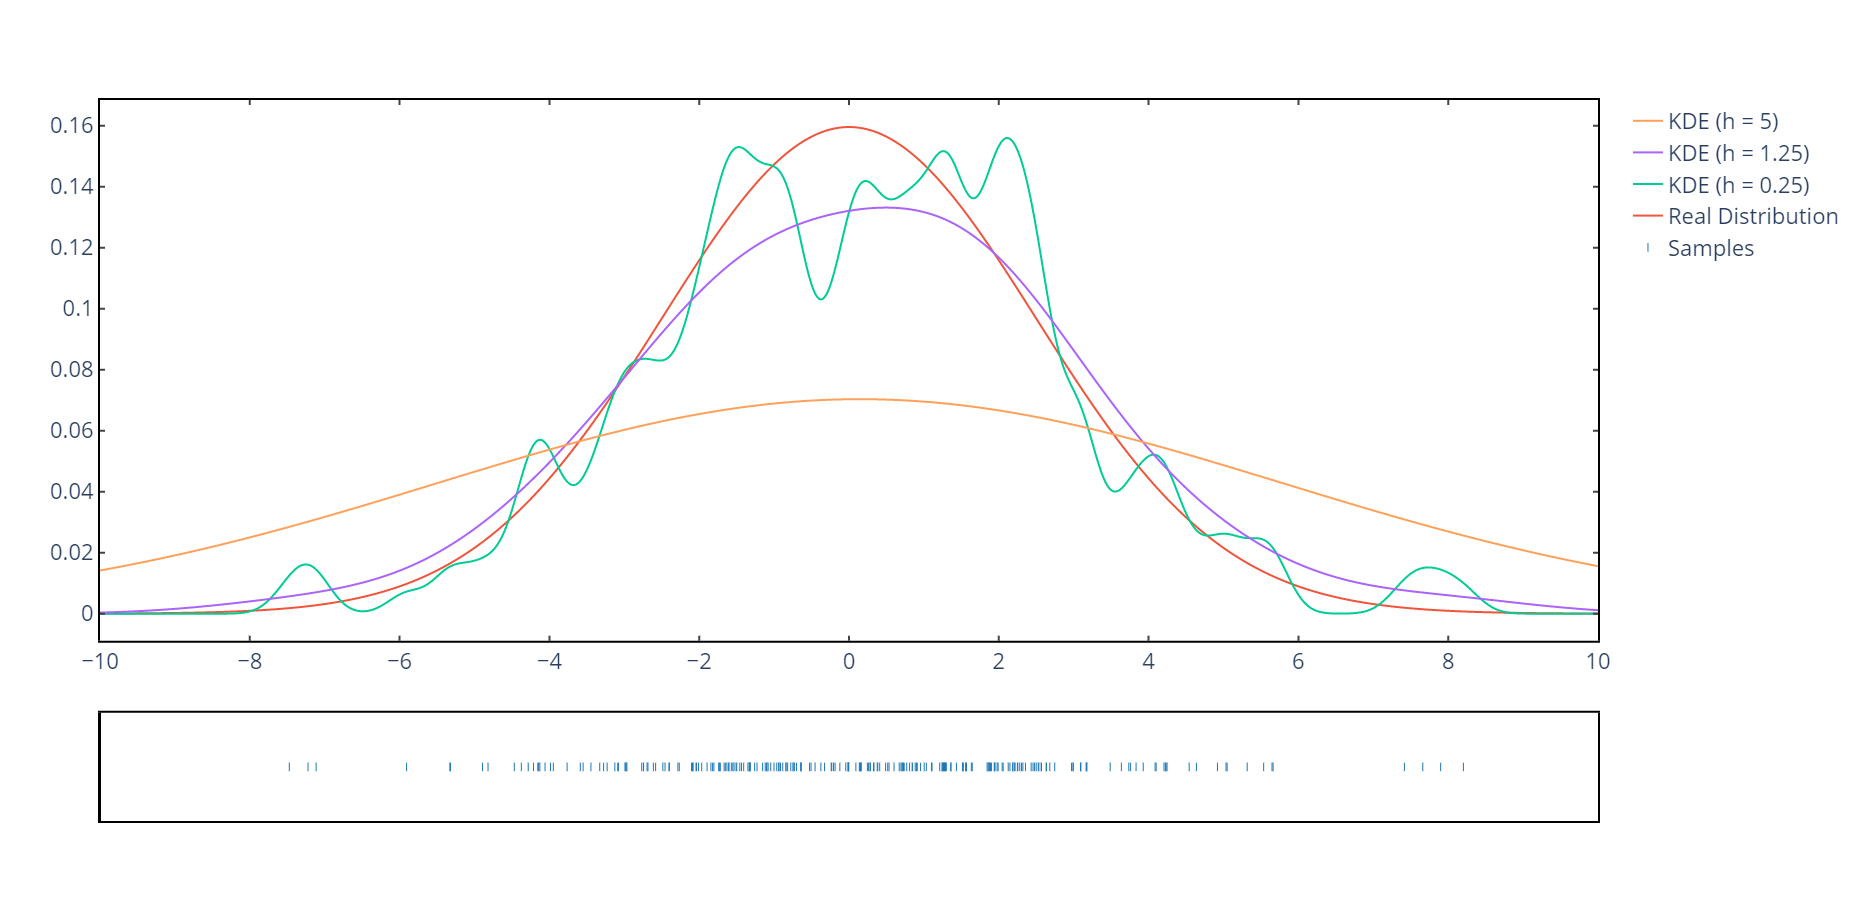
\includegraphics[width=\textwidth]{kde.png}
		\caption{Result of applying KDE with different bandwidths, real distribution and samples are shown}
		\label{fig:kde}
	\end{figure} 

	\textbf{Training:} The Kernel Density Estimator is trained with a number of samples that are stored internally. Additionally, a kernel is selected.
	
	\textbf{Estimation:} To estimate the density at a certain point $x$, the individual centered kernels for every training example $x_i$ are evaluated at the point $x$. Subsequently, the results are summed and scaled to get valid probability values. Equation \ref{eq:kde} shows the full formula.
	
	\begin{equation}
		\label{eq:kde}
		p(x) = \frac{1}{nh}\sum_{i = 1}^{n} k\left(\frac{x - x_i}{h}\right)
	\end{equation}
		
	\subsubsection{Support Vector Machine (SVM)} 
	
	The SVM is a sophisticated classification algorithm trying learn a hyperplane to separate the examples of different classes in the feature space. This is achieved by selecting the hyperplane that yields the largest separation between the classes, i.e. the one that maximizes the distance (the \textit{margin}) to the nearest points of each class. Intuitively, this leads to a better generalization ability to unseen examples, as class separation is maximal. Support Vector Machines are well suited for working with high-dimensional feature spaces and may use a non-linear transformation of data points into an implicit higher-dimensional (and even infinite-dimensional) feature space. This transformation is called a \textit{kernel} (not to be confused with the kernel used in Kernel Density Estimation). 
	
	An advantage of SVMs is the possibility of sparse representation, as only training examples on, within, or on the wrong side of the margin, called \textit{support vectors}, need to be retained for constructing the hyperplane. A cost parameter $C$ penalizes support vectors that are inside the margin or on the wrong side of the hyperplane \cite{Boser1992,Cortes1995}. See Figure \ref{fig:svm} for an example. The possibility of mapping into an implicit higher-dimensional feature space is another advantage when working with data that is not easily separable in the original feature space, but may yield a clear decision boundary in a higher-dimensional space. Disadvantages of SVMS, on the other hand, are the non-trivial selection of parameters that have a huge impact on classification accuracy, the restriction on binary classification problems (using more than two classes requires multiple SVMs) and that the parameters of a trained model can be hard to interpret (cf. \cite{Meyer2003}).
	
	\begin{figure}[tb]
		\centering
		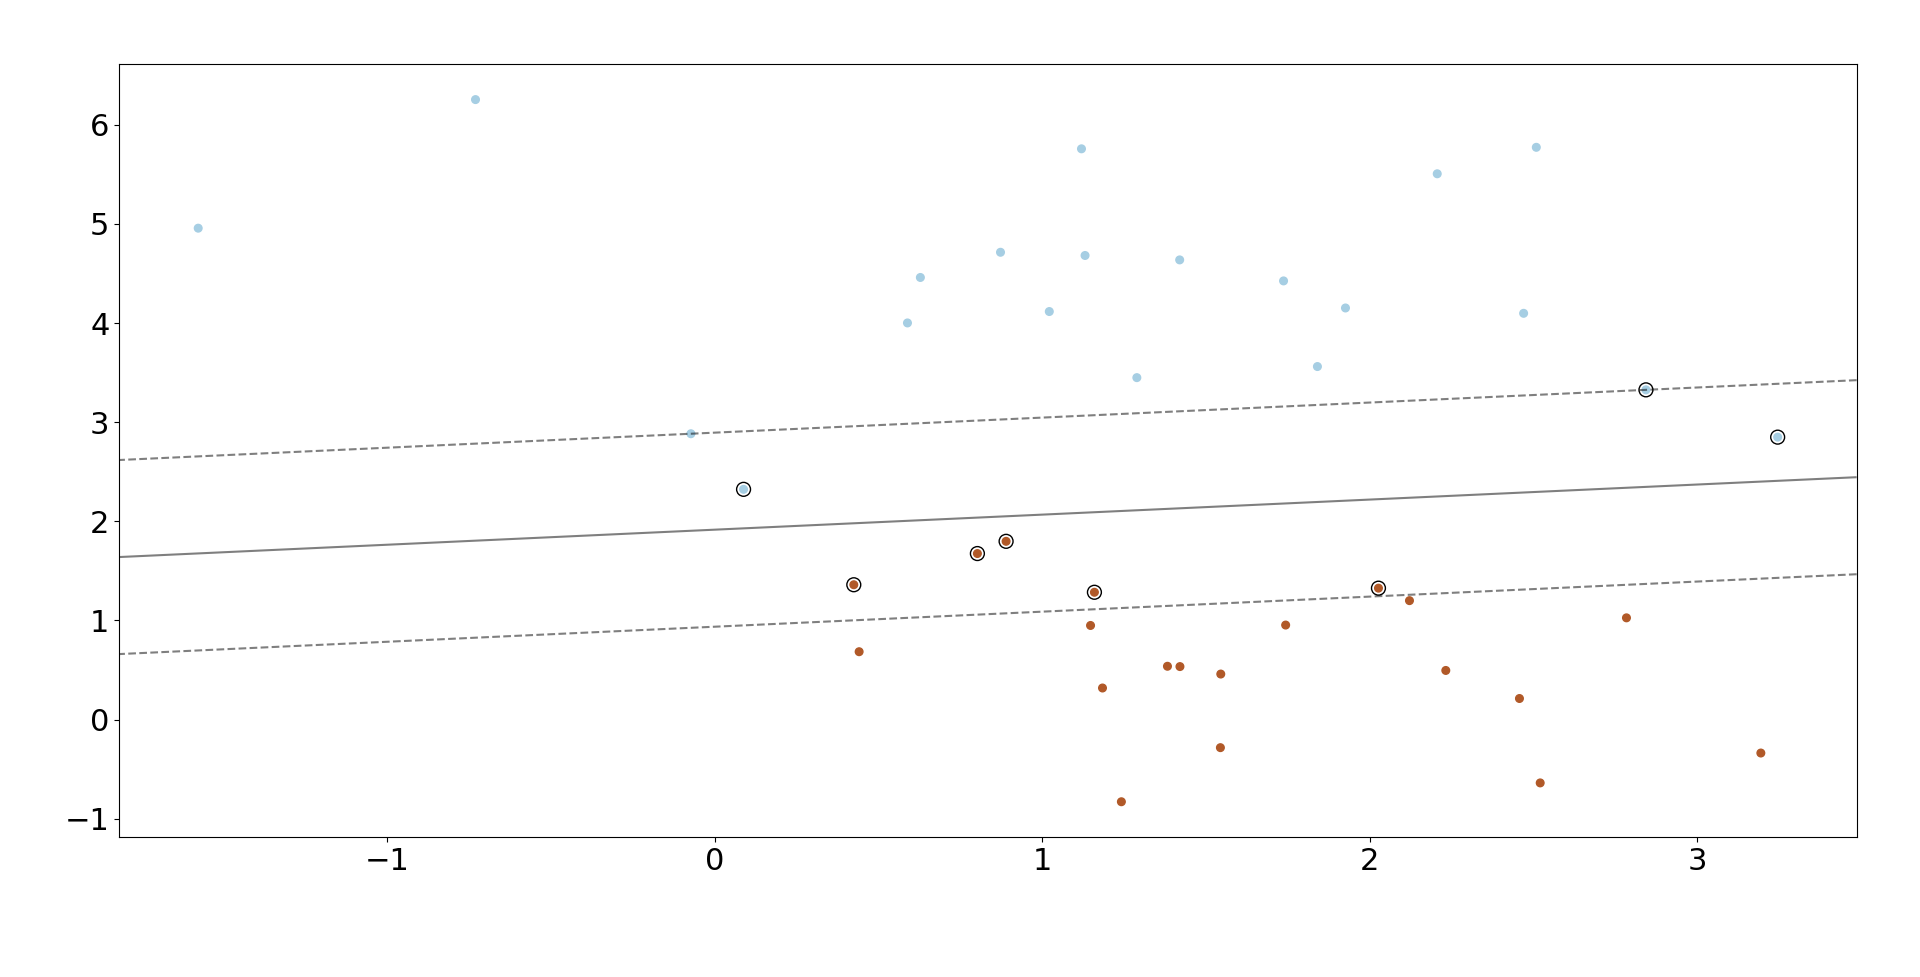
\includegraphics[width=\textwidth]{svm.png}
		\caption{The decision surface of a SVM (with $C = 1$), shown in solid gray and the margin (shown in dashed gray). Training examples are colored by their class, while support vectors are outlined with a black circle (taken from \cite{sklearn-linearSvc} with modifications).}
		\label{fig:svm}
	\end{figure}

	\textbf{Training:} During training, the SVM solves the optimization problem of finding the hyperplane that best separates the data while maximizing the margin. This is done with respect to the penalty parameter $C$. The training examples on or within the margin and on the wrong side of the hyperplane are designated as support vectors. All other training examples may be deleted.
	
	\textbf{Classification:} The separating hyperplane is fully defined given the support vectors. After reconstructing the hyperplane, the example is assigned a class according to on which side of the hyperplane it lies.

	\subsection{Countermeasures}
	\label{theoretical:defenses}

	A defense against WF attacks aims at disguising the identifying patterns in the packet traces the attacker can observe. To this end, packets lengths may be artificially changed, they may be split up into multiple packets, or the timing might be changed. There exist three main classes of defenses, while, naturally, some countermeasures might not fit one particular class, but exhibit characteristics of multiple classes.
	
	\begin{description}
		\item[Padding] Padding schemes are among the simplest countermeasures. They add certain amounts of dummy data to each packet up to the MTU. Padding schemes may be \textit{deterministic} or \textit{probabilistic}, with deterministic schemes always returning the same output trace when presented the same input trace, while this isn't the case for probabilistic padding. When using this type of defense, packets can only grow, but never shrink. Also, packet counts and timing are not affected.
		\item[Noise] Defenses of this class try to disguise the visited web page by deliberately adding noise to the transmission. This can be done for example by loading a second randomly chosen web site in parallel to the requested site \cite{Panchenko2011} or randomizing the order of HTTP requests in the web browser \cite{Perry2011}. Countermeasures using approach may affect packet timing and order and insert new packets into the trace.
		\item[Morphing] Morphing countermeasures are the most complex defenses, trying to hide the actual distribution of packet sizes. They may simply try to make all websites look equal, or at least similar, (cf. \cite{Dyer2012,Cai2014,Cai2014a}) or to make a certain web site look like a different one \cite{Wright2009}. Packet traces may be changed in many ways when using a morphing defense, like adding extra packets, growing or splitting packets, or changing timing.
	\end{description}
	
	\section{Gaussian Padding}
	\label{gaussian_padding}
	
	\textit{Gaussian padding} is a specific form of probabilistic padding. The amount of dummy data added to a packet is drawn from a rounded normal distribution, as opposed to Uniform Padding, where padding sizes are drawn according to the uniform distribution. Furthermore, the tails of the distribution are clipped on both sides, as padding can never take negative values and packets may never become bigger than the MTU. The distribution is parameterized with the desired mean padding size, becoming the mean $\mu$ of the normal distribution. The standard deviation $\sigma$ can be chosen such that the truncated tail corresponds to as little probability mass as desired. For our purpose, choosing $\sigma = \frac{\mu}{3}$ is sufficient, as in this case only approximately $0.1\%$ of the probability mass is allocated to negative values. Figure \ref{fig:trunc_gauss} shows an example distribution function for a truncated rounded normal distribution.
	
	Sampling from a rounded normal distribution is straight-forward by simply sampling from a continuous normal distribution and rounding the value. The truncation can be achieved by rejecting and resampling values that fall out of the desired interval, or by using the method described by Hülsing et al. in \cite{Huelsing2018}, which allows to sample from a rounded Gaussian in constant time, thus mitigating cache timing attacks on the sampling algorithm. While these are out of scope under the threat model of WF, this fact is of particular interest for different fields of research, such as Lattice-based cryptography. \cite{Huelsing2018}
	
	When applying Gaussian padding, the amount of data added to each packet may either be sampled from the distribution independently for each individual packet or once for every session (i.e. page load), leading to \textit{packet-random} Gaussian padding and \textit{session-random} Gaussian padding, respectively.
	
	\begin{figure}[tb]
		\centering
		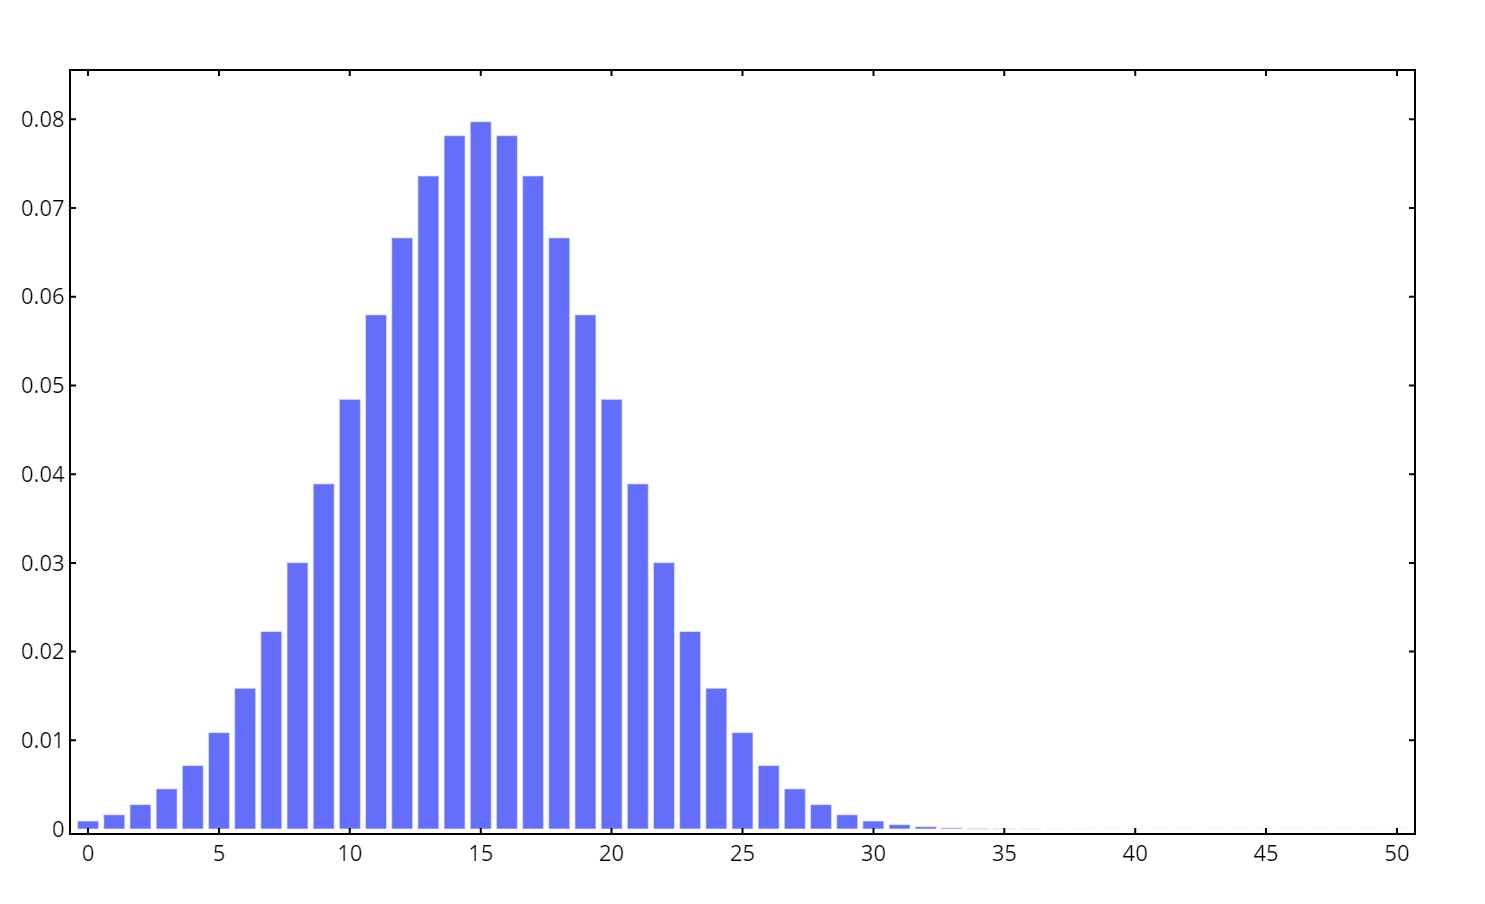
\includegraphics[width=\textwidth]{truncated_rounded_normal.png}
		\caption{An example for a rounded normal distribution, truncated to the left at 0 with a mean padding size of $\mu = 15$ and a standard deviation of $\sigma = 5$ }
		\label{fig:trunc_gauss}
	\end{figure}

	\chapter{Prior Work}
	\label{prior}
	
	Website fingerprinting attacks and defenses have been subject to an "arms race which has continued for more than a decade" \cite{Cherubin2017}. In the following sections, a selection of major WF attacks (Section \ref{prior:attacks}) and defenses (Section \ref{prior:defenses}) are presented. Furthermore, Section \ref{prior:cherubin_bounds} gives an overview over a method proposed by Cherubin \cite{Cherubin2017} to estimate provable security bounds for WF defenses with respect to a given feature set.
	
	\section{Website Fingerprinting Attacks}
	\label{prior:attacks}
	
	Many WF attacks have been published during the last 15 years, with each one improving on the accuracy and performance (including robustness against countermeasures) of the previous attacks. A selection of notable such attacks is presented below, in order of increasing recency. While the early publications still focused on fingerprinting encrypted traffic on SSH tunnels (cf. \cite{Liberatore2006,Herrmann2009,Panchenko2011,Dyer2012}), with the rise in popularity of the Tor anonymization platform\footnote{\url{https://www.torproject.org/}} the focus in the WF community has since shifted heavily towards Tor traffic in the recent years (cf. \cite{Dyer2012,Wang2014,Panchenko2016,Hayes2016,Sirinam2018,Wang2021}). Tor traces pose additional challenges to the attacker, as in Tor all packets have equal length and some countermeasures have already been deployed \cite{Perry2011}. Starting from the \textit{H} attack below, all subsequent attacks are increasingly focused on Tor, with everything beyond \textit{VNG++} no longer considering SSH traffic at all.
	
	\paragraph{LL} In \cite{Liberatore2006}, Liberatore and Levine present two distinct attacks, one based on a modified Jaccard coefficient (a measure for set similarity), and a second one using a Naive Bayes classifier with KDE. While both attacks have been found to yield good results, the Jaccard classifier's accuracy degrades more rapidly in the face of countermeasures \cite{Liberatore2006}. Because of this, most of subsequent work only considered the Naive Bayes classifier, which will be termed \textit{LL} going forward. The attack of Liberatore and Levine uses as features a histogram of packet sizes and directions, i.e. counting the numbers of packets having each size going in each direction. Apart from their contributions to WF attacks, Liberatore and Levine have also published a dataset of website traces for WF evaluation (see Section \ref{methods:dataset} for more details).
	
	\paragraph{H} The attack by Herrmann et al. \cite{Herrmann2009} uses the same feature set as the LL attack, but instead of using the Naive Bayes classifier, it applies a set of well-known text mining transformations on the packet size histogram, namely the \textit{TF (term frequency) transformation} (equation \ref{eq:tf}) and \textit{cosine normalization} (equation \ref{eq:cosine}). Then, they apply the Multinomial Naive Bayes classifier, which is commonly used in text mining \cite{Herrmann2009}. A detailed description of the classifier can be found in \cite[ch. 13]{Manning2008}.
	
	\begin{align}
		f^*_{x_i} &= log(1 + f_{x_i}) \label{eq:tf} \\
		\intertext{The $x_i$ values denote pairs of packet directions and sizes $(d, l) \in \{\uparrow,\downarrow\} \times \{52, \ldots, MTU\}$, while $f_{x_i}$ is the absolute frequency of such packets in the trace. Below, $\|\cdot\|$ denotes the euclidean norm.}
		f^{norm}_{x_i} &= \frac{f^*_{x_i}}{\left\| (f^*_{x_1}, \ldots, f^*_{x_m}) \right\| } \label{eq:cosine}
	\end{align}

	\paragraph{P} A very impactful attack was proposed by Panchenko et al. in \cite{Panchenko2011}. It was one of the first attacks to consider also some coarse-grained features in addition to packet histograms. In particular, information about overall bandwidth, count of distinct packet sizes, fraction of upstream/downstream packets and bursts are added to the feature set. Additionally, they employ a SVM for classification. Altogether, their attack reaches very high accuracy (more than 96\% for 775 websites) even for high class (or, website) counts and has been found robust to many countermeasures \cite{Dyer2012}.
	
	\paragraph{VNG++} In their work in \cite{Dyer2012}, Dyer et al. not only present a comprehensive survey on existing WF attacks and defenses, but also explore the feasibility of website fingerprinting without using a packet histogram, as all previous attacks had been doing. They find that, when using only the overall upload and download bandwidth, the total transmission time and a burst size histogram, results similar to that of the P attack can be achieved while using a Naive Bayes classifier with KDE. Dyer et al. also note that, using the same feature set as the P attack, but the NB classifier instead of a SVM, performance doesn't degrade much from the original P attack, suggesting that using a complex classification algorithm isn't necessary to obtain good results in WF \cite{Dyer2012}.
	
	\paragraph{$k$-NN} Wang et al. \cite{Wang2014} further developed the idea of using a simple classification algorithm by resorting to the $k$-NN classifier and choosing a large set of different features, including total bandwidth and transmission time, occurrence of unique packet sizes, information on packet ordering and bursts (although with a slightly different definition than the one that was given earlier) as well as the size and direction of the first 20 packets in each trace. Furthermore, they determine weights for all features signifying their relative importance, which are multiplied with the feature vectors prior to classification. For the detailed description of the algorithms, refer to \cite{Wang2014}.
	
	\paragraph{CUMUL} A more recent contribution of Panchenko et al. \cite{Panchenko2016}, the CUMUL attack also uses a SVM classifier, like the P attack did before. While Wang et al. used a multitude of manually selected features in their $k$-NN attack (up to 4000), Panchenko et al. focus on creating an abstract representation that implicitly covers the characteristics of a page load \cite{Wang2014,Panchenko2016}. In addition to the basic features of packet count and bandwidth per direction, they create a cumulative sum of the packet sequence (with outgoing packets having negative size) and sample a fixed number $n$ of additional features from this cumulative sum using linear interpolation. In their work, Panchenko et al. find $n = 100$ to yield good results, leading to only 104 features in total \cite{Panchenko2016}.
	
	\paragraph{Recent Attacks} Many more attacks have been published in recent years which are mentioned here for the sake of completeness. Hayes and Danezis published the $k$-FP (or $k$-Fingerprinting) attack where they are using a modified Random Forest classifier to extract an abstract fingerprint for each website, which is then classified using the $k$-NN classifier \cite{Hayes2016}. Sirinam et al. employ deep learning techniques, namely Convolutional Neural Networks (CNN), to website fingerprinting, yielding the DF (Deep Fingerprinting) attack \cite{Sirinam2018}. Later, Wang et al. proposed the Adaptive Fingerprinting (AF) attack, greatly reducing the amount of data needed to train the deep learning algorithms\footnote{Usually, deep learning algorithms require a very large amount of training data due to their complex nature and slow optimization convergence}. At the same time, AF reduces the need to frequently update the training data due to the sensitivity to content changes of contained websites \cite{Wang2021}.
	
	\section{Website Fingerprinting Defenses}
	\label{prior:defenses}
	
	In the following, a number of major WF defenses from all the three classes (cf. Section \ref{theoretical:defenses}) will be briefly presented.
	
	\paragraph{Classical Padding Defenses} There are a multitude of padding schemes that can be applied to the WF setting, some of which are deterministic and some probabilistic. A good overview of them is given in \cite{Dyer2012}. Table \ref{tbl:padding} also shows a selection of them.
	
	\begin{table}
		\centering
		\small
		\begin{tabularx}{\textwidth}{llX}
			\toprule \textbf{Name} & \textbf{Type} & \textbf{Description} \\
			\midrule Linear Padding & deterministic & pad to the next multiple of 128 bytes, or the MTU \\
			Exponential Padding & deterministic & pad to the next power of two, or the MTU \\
			Mice-Elephants & deterministic & pad to 128 bytes if the packet has $l \leq 128$, or otherwise to the MTU \\
			Pad to MTU & deterministic & Each packet size is increased to the MTU \\ \addlinespace 
			Session Random 255 & probabilistic & Sample a value $r \in \{0, 8, 16, ..., 248\}$ uniformly at random for the session. Increase each packet length by this amount. \\
			Packet Random 255 & probabilistic & Sample a value $r \in \{0, 8, 16, ..., 248\}$ uniformly at random for each packet. Increase the packet length by this amount. \\
			\bottomrule
		\end{tabularx}
		\caption{An overview of classical padding schemes that have been applied to website fingerprinting \cite{Dyer2012}}
		\label{tbl:padding}
	\end{table}

	\paragraph{Defense by Noise} Several defenses using noise to disguise a website's identifying patterns have been proposed in the past. One notable examples are \textit{Decoy Pages}, as proposed by Panchenko et al. in \cite{Panchenko2011}, where a random webpage is loaded in parallel to the desired web page, thus producing noise through unrelated traffic. Another such defense is \textit{Randomized Pipelining}, as deployed in the Tor Browser, which randomizes the order of parallel HTTP requests sent over the same connection (HTTP pipelining) \cite{Perry2011,Cherubin2017}.
	
	\paragraph{Morphing Defenses} One of the first publications studying morphing defenses is the \textit{Traffic Morphing} algorithm by Wright et al. \cite{Wright2009}. This defense tries to make web pages look like other pages by learning a so-called \textit{morphing matrix} that transforms the packet size distribution (\textit{source distribution}) such that it resembles the distribution of a different web page (\textit{target distribution}). The morphing matrix is learned using convex optimization to maximize the similarity between the source and target distributions while keeping the overhead minimal. During the process, packets may be split and resized to match the target distribution best. Another similar algorithm presented by Dyer et al. in \cite{Dyer2012} is called \textit{Direct Target Sampling}, where the complex morphing step is skipped and target packet sizes are sampled directly from the selected target distribution.
	
	Another class of morphing defenses aims at reducing differences between the traces of different websites, thus making it harder to distinguish them. They try to limit information available to the attacker. Examples for such defenses are shown in Table \ref{tbl:morphing}.
	
	\begin{table}
		\centering
		\begin{tabularx}{\textwidth}{llX}
			\toprule \textbf{Name} & \textbf{Authors} & \textbf{Description} \\
			\midrule BuFLO & Dyer et al. \cite{Dyer2012} & Sends packets of fixed size $d$ at a fixed interval $\rho$ for at least a fixed time $\tau$, introducing dummy packets when needed \\
			Tamaraw & Cai et al. \cite{Cai2014} & Sends packets of fixed size $d$ at fixed intervals, while the interval $\rho_{out}$ for outgoing packets and $\rho_{in}$ for incoming packets are distinct and $\rho_{out} > \rho_{in}$. Pads the number of packets in either direction by multiples of a parameter. \cite{Cherubin2017} \\
			CS-BuFLO & Cai et al. \cite{Cai2014a} & Similar to BuFLO, but adapts $\rho$ to the available network bandwidth dynamically. \\
			\bottomrule
		\end{tabularx}
		\caption{Examples for morphing defenses trying to reduce information available to the attacker}
		\label{tbl:morphing}
	\end{table}
			
	\section[Security Bound Estimation]{Security Bound Estimation According to Cherubin \cite{Cherubin2017}}
	\label{prior:cherubin_bounds}
	
	When evaluating WF attacks and defenses, the traditional approach is to empirically measure their performance on a previously collected data set of packet traces. However, such empirical
	evaluations are susceptible to noise and fail to produce provable statements on the security of
	a certain defense. While a defense may perform particularly well against the attacks it is evaluated on, it may just as well horribly fail on a different attack that wasn't considered yet. To address this problem and further advance research on provable security evaluation of WF defenses, Cherubin introduces a novel method centered around the Bayes error in \cite{Cherubin2017}.
	
	The \textit{Bayes error} is defined as the minimum probability of error that any classifier can commit given a joint probability distribution on the features and class labels.  Intuitively speaking, the Bayes error corresponds to the area of uncertainty in the probability distribution, i.e. the area where the conditional probabilities $p(x \mid c_i)$ and $p(x \mid c_j)$ overlap\footnote{That is, both probabilities are non-zero} for any two classes $c_i \neq c_j$ and features $x$. 
	
	To formalize, let $\mathcal{X}$ be the feature space and $\mathcal{C}$ the set of all class labels. Let $p(x, c)$ be a joint probability distribution on $\mathcal{X}\times\mathcal{C}$. Then for the set of classifiers $\mathcal{F} = \{f \mid f : \mathcal{X} \to \mathcal{C}\}$ with $R_f$ being the error of a classifier $f\in\mathcal{F}$ according to $p$, the Bayes error $R^*$ is defined as
	
	\begin{align}
		R^* &= \min_{f\in\mathcal{F}} R_f
		\intertext{This minimum error is achieved by the \textit{Bayes classifier} $f^*\in\mathcal{F}$ that assigns to each example $x$ the class label $c$ maximizing the probability $p(c \mid x)$ \cite{Duda2000}.}
		f^*(x) &= \arg\max_{c\in\mathcal{C}} p(c \mid x) \\
		R^* &= R_{f^*}
	\end{align}
	
	As the true joint probability distribution $p(x, c)$ is typically not known in practice, the exact value of the Bayes error can't be calculated. However, there are well-known methods to estimate a lower bound for the Bayes error. Cherubin uses an estimate based on the NN classifier (see Section \ref{ml:nn}) first presented by Cover and Hart \cite{Cover1967} deriving a lower bound $\widehat{R}^*$ for the Bayes error $R^*$
	
	\begin{equation}
		\widehat{R}^* = \frac{L - 1}{L} \left(1 - \sqrt{1 - \frac{L}{L-1}\widehat{R}_{NN}}\right) \leq R^*
		\label{eq:bayes_error_bound}
	\end{equation}
	
	where $\widehat{R}_{NN}$ is the empirical error of the NN classifier on a data set containing $L = |\mathcal{C}|$ classes.
	
	Apart from the lower error bound $\widehat{R}^*$, Cherubin defines an additional privacy metric, called $\varepsilon$-privacy, that is based on the advantage of an adversary. The advantage denotes how much better the adversary can do than random guessing. It is typically defined in a two-class setting, but can be extended to the multi-class classification with $L$ classes \cite{Cherubin2017}. Let $R_G$ be the random guessing error. Then, the advantage $Adv$ is defined as
	
	\begin{align}
		R_G &= \frac{L-1}{L}\\
		Adv &= \frac{1}{R_G}|R_G - \widehat{R}^*|
		\intertext{Cherubin now defines a privacy measure from the advantage:}
		\varepsilon &= 1 - Adv
		\intertext{Given the assumption that $\widehat{R}^* \leq R_G$, this simplifies to}
		\varepsilon &= \frac{\widehat{R}^*}{R_G}
		\label{eq:epsilon}
	\end{align}

	$\varepsilon$ can take values from $[0, 1]$, where $\varepsilon = 1$ stands for the perfect defense which guarantees that an adversary can never do better than random guessing, while $\varepsilon = 0$ means that the adversary always achieves perfect accuracy. 

	\chapter{Experimental Methodology}
	\label{methods}
	\IMRADlabel{methods}

	\section{Trace Data}
	\label{methods:dataset}

	In this work, the data set collected by Liberatore and Levine in \cite{Liberatore2006}, called the \textit{Liberatore data set} in the following, was used for all experiments\footnote{The traces are publicly available under \url{http://traces.cs.umass.edu/}}. The data set contains 2000 distinct web sites sampled from the university department's internet traffic and 205 traces per website. 
	
	Although Herrmann et al. \cite{Herrmann2009} also published a trace data set that was subsequently used in multiple publications (cf. \cite{Panchenko2011,Dyer2012}) and is considered to be of higher overall quality \cite{Dyer2012}, it was no longer accessible under the URL given in their paper, so it couldn't be used here. There were several preprocessing steps done to achieve better data quality. In the following sections, an overview of the main issues in the data set (Section \ref{methods:dataset:quality}) is given and the preprocessing (Section \ref{methods:dataset:pre}) is described.
	
	\subsection{Data Quality}
	\label{methods:dataset:quality}
	
	Several issues have become apparent during the use of the Liberatore data set, which demanded careful preprocessing to clean as much inherently inconsistent data as possible. First of all, there were many traces that didn't contain a single packet in either direction. Some websites even didn't have a single trace that contained a packet. Furthermore, some traces only consisted of a single 52 byte packet, which corresponds to a single \texttt{ACK}. Such traces clearly don't represent a properly recorded page load and are thus counterproductive to the classification task that is website fingerprinting. According to Dyer et al. \cite{Dyer2012}, 13.8\% of the traces in the Liberatore data set are having 10 packets or less in both directions combined, which is highly improbable for most websites. An overview of other statistical properties of the data set is shown in Table \ref{tbl:dataset_props}.
	
	\begin{table}
		\centering
		\begin{tabularx}{0.7\textwidth}{Xr}
			\toprule Traces with 0 packets in one direction & 3.1\% \\
			Traces with $\leq 5$ bidirectional packets & 5.2\% \\
			Traces with $\leq 10$ bidirectional packets & 13.8\% \\
			Traces with $\leq 1\,\text{s}$ duration & 29.4\% \\
			Median trace duration & 2.4$\,\text{s}$ \\
			Median bidirectional packet count & 106 \\
			Median overall bandwidth utilization & 78,382$\,\text{byte}$ \\
			\bottomrule
		\end{tabularx}
		\caption{Statistical properties of the Liberatore dataset \cite{Liberatore2006}, taken from \cite{Dyer2012}}
		\label{tbl:dataset_props}
	\end{table} 
	
	Another irregularity that was observed came with the fact that some traces have an incoming packet as the first one recorded. This behavior is entirely unexpected in the context of loading a web page, as the client first needs to make a HTTP request before the server will send any data back.
	
	Furthermore, there were some clear outliers in the trace data that probably correspond to incomplete page loads. Such outliers may negatively affect classification accuracy. An example for such an outlier is shown in Table \ref{tbl:outlier}.
	
	\begin{table}
		\centering
		\begin{tabular}{lrrrr}
			\toprule & \multicolumn{2}{c}{\textbf{Incoming}} & \multicolumn{2}{c}{\textbf{Outgoing}} \\
			\textbf{Trace ID} & \textbf{Bandwidth} & \textbf{Packets} & \textbf{Bandwidth} & \textbf{Packets} \\
			\midrule 65 & 68,052$\,\text{byte}$ & 81 & 8,140$\,\text{byte}$ & 19 \\
			66 & 68,256$\,\text{byte}$ & 84 & 8,140$\,\text{byte}$ & 19 \\
			67 & 5,968$\,\text{byte}$ & 8 & 1,312$\,\text{byte}$ & 4 \\
			68 & 67,724$\,\text{byte}$ & 75 & 8,596$\,\text{byte}$ & 17 \\
			69 & 67,880$\,\text{byte}$ & 78 & 8,140$\,\text{byte}$ & 19 \\
			\bottomrule
		\end{tabular}
		\caption[An outlier in trace data]{An outlier in trace data. Data for web page \#1156 is shown with traces \#65-\#69. Trace \#67 clearly deviates from the majority of other traces. For the data shown, \texttt{ACK} packets (all packets sized $52\,\text{byte}$) were filtered.}
		\label{tbl:outlier}
	\end{table}

	\subsection{Preprocessing}
	\label{methods:dataset:pre}
	
	To eliminate as much anomalies as possible before running evaluations on the data, it was analyzed thoroughly using outlier detection to filter out pages with a high fraction of degenerate traces as described in the previous section. Three separate outlier detection methods have been combined to form an ensemble outlier detector, which serves to draw conclusions on possible outliers with a higher certainty than when using only a single detection method. Prior to outlier detection, simple \texttt{ACK} packets (all packets sized $52\,\text{byte}$) were filtered from all traces to reduce noise and focus on actual payload transmitted over the network. Then, traces were aggregated to obtain the utilized bandwidth and packet count in either direction, which yields four dimensions per trace. For outlier detection, three detectors implemented in the \texttt{scikit-learn}\footnote{\url{https://scikit-learn.org/}} package \cite{Pedregosa2011} were used, namely the \texttt{EllipticEnvelope}, \texttt{LocalOutlierFactor} and \texttt{IsolationForest} algorithms\footnote{For details on the algorithms, please refer to \url{https://scikit-learn.org/stable/modules/outlier_detection.html}}. The output of these detectors is either 1 or -1, marking an inlier or outlier, respectively. Let $o_{env}, o_{lof}, o_{ilf} \in \{-1, 1\}$ be the output of the three detectors. Then, an outlier score $o$ can be defined as
	
	\begin{align*}
		o &= o_{env} +  o_{lof} + o_{ilf}
		\intertext{$o$ can only take values $\{-3, -1, 1, 3\}$, which is then mapped to the outlier decision $o^*$ as follows}
		o^* &= \begin{cases}
			\text{inlier}, &o = 3,\\
			\text{probable inlier}, &o = 1,\\
			\text{probable outlier}, &o = -1,\\
			\text{outlier}, &o = -3.
		\end{cases}
	\end{align*}

	This evaluation leads to the conclusion that roughly 11.9\% of the traces in the data set are outliers or probable outliers with respect to the previous detection method. The distribution of the count of traces per website for which $o^* \in \{\text{outlier}, \text{probable outlier}\}$ has the properties shown in Table \ref{tbl:outlier_dist}.
	
	\begin{table}
		\centering
		\begin{tabular}{lrr}
			\toprule & \textbf{Before Preprocessing} & \textbf{After Preprocessing} \\
			\midrule Mean & 24.32 & 20.61 \\
			Standard Deviation & 8.80 & 5.22 \\
			Minimum & 0 & 1\\
			25\% Percentile & 19 & 18 \\
			Median & 24 & 21 \\
			75\% Percentile & 29 & 24 \\
			Maximum & 63 & 31\\
			\bottomrule
		\end{tabular}
		\caption{The distribution of outlier or probable outlier count per website}
		\label{tbl:outlier_dist}
	\end{table}

	After analyzing the outlier traces, the data set was filtered using two criteria:
	
	\begin{enumerate}
		\item Drop all websites having 29 or more outlier traces, thus keeping the 75\% percentile of the data in regard to outlier count.
		\item From the remaining websites drop all that have at least one trace with three or fewer packets in both directions. Traces that have three or fewer packets in one direction, but more than three in the other one are not considered.
	\end{enumerate}

	After these preprocessing steps, 532 websites out of the initial 2000 remain in the data set. The changed outlier characteristics can be viewed in Table \ref{tbl:outlier_dist}. The mean number of outliers or probably outliers per website went down to 20.61 from 24.32, thus lowering the outlier rate to 10.1\%. Note that many of the websites with low outlier count were degenerate with respect to the packet count filter, in the sense that the majority of their traces had zero or only one packet, which is the reason why the average outlier count couldn't be lowered more significantly. Nonetheless, the outlier characteristics were clearly improved through preprocessing.

	\section{Evaluating Attack Performance}
	\label{pipeline}
	
	Attacks and defenses were evaluated against each other using a generic framework implemented in the course of this thesis, which provides a generic evaluation pipeline. It consists of four stages, which are briefly described in the following sections. All implementations were done in Python 3.8 using the \texttt{scikit-learn} machine learning toolkit \cite{Pedregosa2011}, as well as the \texttt{numpy}\footnote{\url{https://numpy.org/}} \cite{Harris2020} and \texttt{scipy}\footnote{\url{https://www.scipy.org/}} \cite{Virtanen2020} libraries for scientific computing and \texttt{pandas}\footnote{\url{https://pandas.pydata.org/}} \cite{McKinney2010,Reback2021} for data manipulation and I/O. APIs have been modeled after the example of \texttt{scikit-learn} \cite{Buitinck2013} where possible.
	
	An instance of the pipeline is always ran with a set of training and a set of test data, which are distinct. It may run multiple evaluations for different attacks and defenses in parallel, for which the \texttt{multiprocessing} module from Python's standard library is utilized. The number of training and test examples to use for evaluation as well as the offset between training and test data can be customized. For all experiments, the offset between training and test data was set to 0, i.e. both sets are read from a single contiguous range of trace IDs. The first trace id of this set was randomized. Varying numbers of training examples had to be used, following the previous author's suggestions. See Table \ref{tbl:train} for the exact numbers. The number of test examples per website was always set to be 4.
	
	\begin{table}
		\centering
		\begin{tabularx}{0.85\textwidth}{lXr}
			\toprule \textbf{Attack} & \textbf{Authors} & \textbf{Training Examples} \\
			\midrule LL & Liberatore \& Levine \cite{Liberatore2006} & 4 \\
			H & Herrmann et al. \cite{Herrmann2009} & 4 \\
			P & Panchenko et al. \cite{Panchenko2011} & 18\\
			VNG++ & Dyer et al. \cite{Dyer2012} & 16${}^*$\\
			CUMUL & Panchenko et al. \cite{Panchenko2016} & 45${}^\dagger$\\
			\bottomrule
		\end{tabularx}
		\caption[The number of training examples used for each attack]{The number of training examples used for each attack.\\{*} = For VNG++, Dyer et al. did not specify the number they used in their publication, therefore the default setting from their published source code was used.\\{${}^\dagger$} = For CUMUL the number of training examples was chosen that yielded the best accuracy on average}
		\label{tbl:train}
	\end{table}
	
	\subsection{Data Set}
	
	The data set stage takes care of loading traces and abstracts from the storage technology used for the data set. It mainly consists of an implementation of the abstract class \texttt{Dataset} encapsulating all logic required to load a dataset and transform it into a \texttt{pandas} data frame with the following columns, where each row corresponds to a recorded packet:
	
	\begin{itemize}
		\item \texttt{site\_id}: The ID of the website, must be unique within the data set
		\item \texttt{trace\_id}: The ID of the packet trace, must be unique within the same website
		\item \texttt{collection\_time}: The time at which the trace collection started
		\item \texttt{time}: The offset of the packet's arrival from the first packet in the trace in milliseconds
		\item \texttt{size}: The length of the packet, negative for outgoing packets and positive for incoming packets
	\end{itemize}

	An implementation is provided for the Liberatore dataset, containing additional functionality to download, extract and parse the PCAP logs of the data set and store them in the HDF5 format for quick and easy access.
	
	\subsection{Defense}
	
	After the data set follows the optional defense stage, which is only present when attacks should be evaluated against defenses. This stage is implemented using the \texttt{Defense} class, which takes packet traces in the format as returned by \texttt{Dataset} and returns the same data structure. Defenses normally change the \texttt{size} and/or \texttt{time} columns of a trace.
	
	Implementations of all padding defenses mentioned in Section \ref{prior:defenses} are provided, as well as Gaussian padding in packet-random and session-random mode.
	
	\subsection{Feature Extraction}
	
	In the feature extraction stage, packet traces are transformed to a single vector of features and a class label (the \texttt{site\_id}). The output of this stage is no longer expected to be a \texttt{pandas} dataframe, but a pair of \texttt{numpy} arrays, the first containing all feature values and the second containing the class labels.
	
	Individual feature sets can be combined using the features from both sets and transformed, using any \texttt{scikit-learn} transformer, as done with the TF transformation and cosine normalization in the attack by Herrmann et al. \cite{Herrmann2009}.
	
	The framework created during this thesis provides implementations for the feature sets of Liberatore and Levine \cite{Liberatore2006}, Herrmann et al. \cite{Herrmann2009}, Panchenko et al. \cite{Panchenko2011, Panchenko2016} and Dyer et al. \cite{Dyer2012}. Most operations have been implemented solely as \texttt{numpy} array operations and \texttt{pandas} aggregations due to the superior speed because of them running in native C code \cite{Harris2020,McKinney2010}.
	
	\subsection{Classifier}
	
	The final stage of the pipeline is a classifier which is trained using the features and class labels extracted from the training data. Then, the test data's features are classified with the trained classifier and the chosen performance measure is calculated using the predicted classes against the actual class labels. The default and most common choice for said performance measure is accuracy (the fraction of correctly classified examples).
	
	All classification algorithms have been implemented using \texttt{scikit-learn}. For Multinomial Naive Bayes and SVM the implementations provided by the library were used. Unfortunately, it doesn't contain an implementation of Naive Bayes using Kernel Density Estimation, so that variant was implemented following \texttt{scikit-learn}'s typical API design \cite{Buitinck2013}. Also, an efficient variant of one-dimensional KDE was implemented following the algorithm from the WEKA Java machine learning toolkit\footnote{\url{https://www.cs.waikato.ac.nz/ml/weka/}} \cite{Frank2016}, which was used by most prior publications that were using the NB classifier with KDE (cf. \cite{Liberatore2006,Dyer2012}).

	\section{Error Bound Estimation}
	\label{error_bound_estimation}

	When estimating lower bounds for classifier error according to the method developed by Cherubin \cite{Cherubin2017}, the general flow and pipeline structure resembles closely the one described in the previous section. However, as the final stage of the pipeline, the attack's classifier is substituted by Cherubin's error estimator. Also, there are no distinct training and test sets in this pipeline as the estimator calculates the accuracy of the NN classifier using 5-fold cross validation (CV). In this method, the data set is split up into five equal parts, of which each one serves as the test set once while the other four become the training set. After measuring the classification accuracy for all five runs, the results are averaged to obtain a final score.
	
	For this evaluation, 100 websites were used with 100 traces each which were loaded from a contiguous range of trace IDs. The first trace ID of the data set was randomized. The experiment was repeated 50 times for both, the closed-world and open-world mode (see below).
	
	\subsection{Bayes Error Estimator}
	
	The Bayes error estimator operates either in closed-world or open-world mode. In closed-world, the data set received is directly split up for cross validation and accuracy is measured using all websites and traces. In contrast, when using the open-world mode, for each website present in the data, all traces of that website and exactly as many randomly selected traces of different websites are passed on to the cross validation. This corresponds to the One-vs-All mode described by Cherubin \cite{Cherubin2017}, in which the monitoring of a single website against all others is simulated.
	
	After calculating the CV accuracy, the formula from Equation \ref{eq:bayes_error_bound} is used to calculate $\widehat{R}^*$ as the lower bound of the Bayes error. From that, the privacy measure $\varepsilon$ is calculated as shown in Equation \ref{eq:epsilon}.

	\chapter{Results}
	\label{results}
	\IMRADlabel{results}
	
	During the experiments, a modified version of the Packet Random 255 and Session Random 255 defenses was used, called Packet Random Uniform and Session Random Uniform. The modification was extending the set from which padding is drawn to be $\{0, 8, 16, 24, \ldots, 256\}$. The expected value for the Gaussian padding distribution was chosen to be $\mu = 128$, as to fit the expected value of the uniform distribution.
	
	Using the evaluation pipelines described in the previous section, there were three experiments run. In each experiment, the defenses Packet Random Uniform, Session Random Uniform, Packet Random Gaussian and Session Random Gaussian were evaluated against the LL, H, P, VNG++ and CUMUL attacks. Additionally, the attacks were evaluated without a defense to obtain a baseline performance. The following experiments were carried out:
	
	\begin{enumerate}
		\item Evaluate attack performance for $n \in \{2, 4, 8, 16, \ldots, 512\}$ randomly selected websites. For each pair of attack and defense and each $n$, the evaluation was run 10 times.
		\item Evaluate attack performance for $n = 128$ randomly selected websites. For each pair of attack and defense the evaluation was run 50 times.
		\item Estimate $\widehat{R}^*$ and $\varepsilon$ for each defense. The estimation was run 50 times on 128 randomly selected websites and 100 traces per site. For each pair of attack and defense error bounds were calculated in both, the closed world and the open world (one-vs-all) scenario.
	\end{enumerate}

	\section{Empirical Performance of Gaussian Padding}
	\label{performance}
	
	Figures \ref{fig:ll}, \ref{fig:h}, \ref{fig:p} and \ref{fig:vng++} display the performance of the LL, H, P and VNG++ attacks against the random padding defenses, respectively. One major thing to notice is that Gaussian padding works particularly well against the LL and H attacks, while it largely fails to thwart the attacks against P and VNG++. Especially the VNG++ classifier is robust against both randomized padding schemes, as it experiences the smallest drop in accuracy, only about 5\% at $n = 512$. In contrast, the accuracy of the P classifier drops by approximately 25\% for both session random schemes, but still achieves an accuracy of 60\%. Much differently, the LL and H attacks only manage under 5\% of accuracy against the best defense at $n = 400$.
	
	A second notable thing is the difference between packet random and session random padding schemes. For all attacks that have been evaluated, session random padding performs considerably better. Against the P attack this difference is particularly large, reaching close to 10\% difference in accuracy. That said, the efficiency gap is smaller for all other attacks, although still noticeable. VNG++ has the 
	
	When comparing Gaussian padding with uniform padding, it stands out that for some attacks there's a clear advantage of Gaussian padding over the uniform variant, while for others, they seem to perform almost equally or with a slight advantage for uniform padding. Considering the P attack, the padding distributions can only hardly be distinguished, yielding almost identical performance in both, the packet random and session random schemes. On the other hand, against the LL and H attacks, Gaussian padding clearly performs better up to a difference of more than 5\% in classifier accuracy for the session random scheme. Finally, in the VNG++ attack, uniform and Gaussian padding are exhibiting very similar performance, with a perceived small advantage for uniform padding.

	\begin{figure}
		\begin{subfigure}{0.495\textwidth}
			\centering
			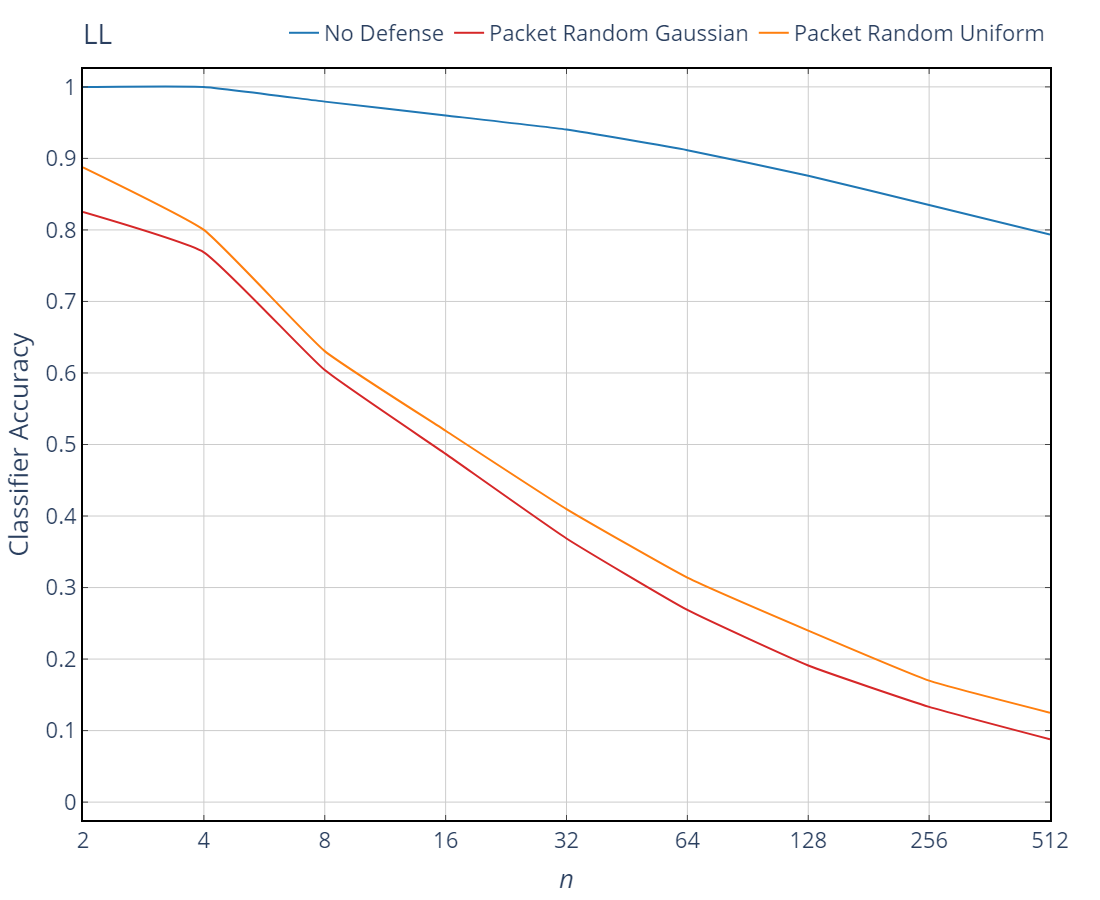
\includegraphics[width=\textwidth]{plots/performance_ll_pkt.png}
			\caption{Packet Random Padding}
		\end{subfigure}
		\hfill
		\begin{subfigure}{0.495\textwidth}
			\centering
			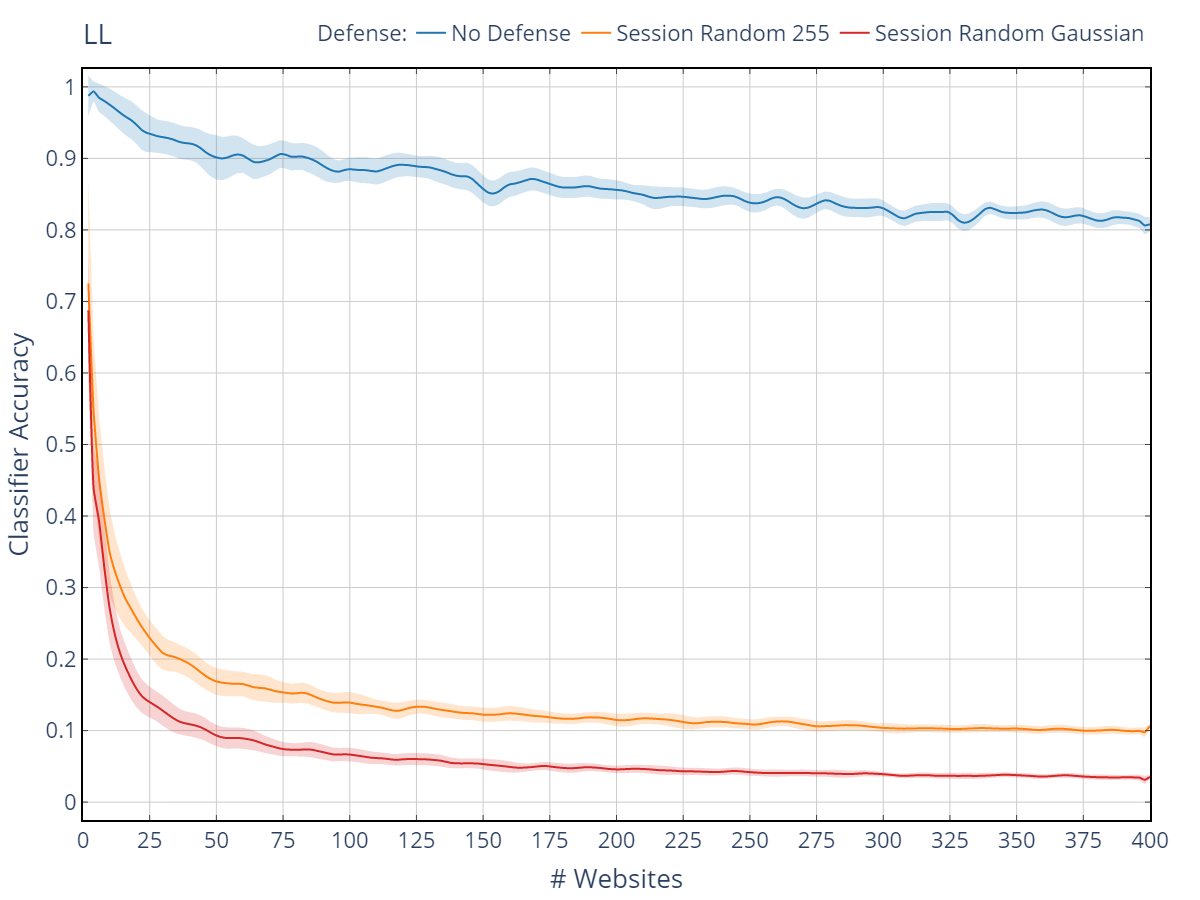
\includegraphics[width=\textwidth]{plots/performance_ll_ses.png}
			\caption{Session Random Padding}
		\end{subfigure}
		\caption[Performance of Gaussian padding against the LL attack]{Performance of Gaussian padding against the LL attack \cite{Liberatore2006} in comparison to uniform padding.}
		\label{fig:ll}
	\end{figure}
	\begin{figure}
		\begin{subfigure}{0.495\textwidth}
			\centering
			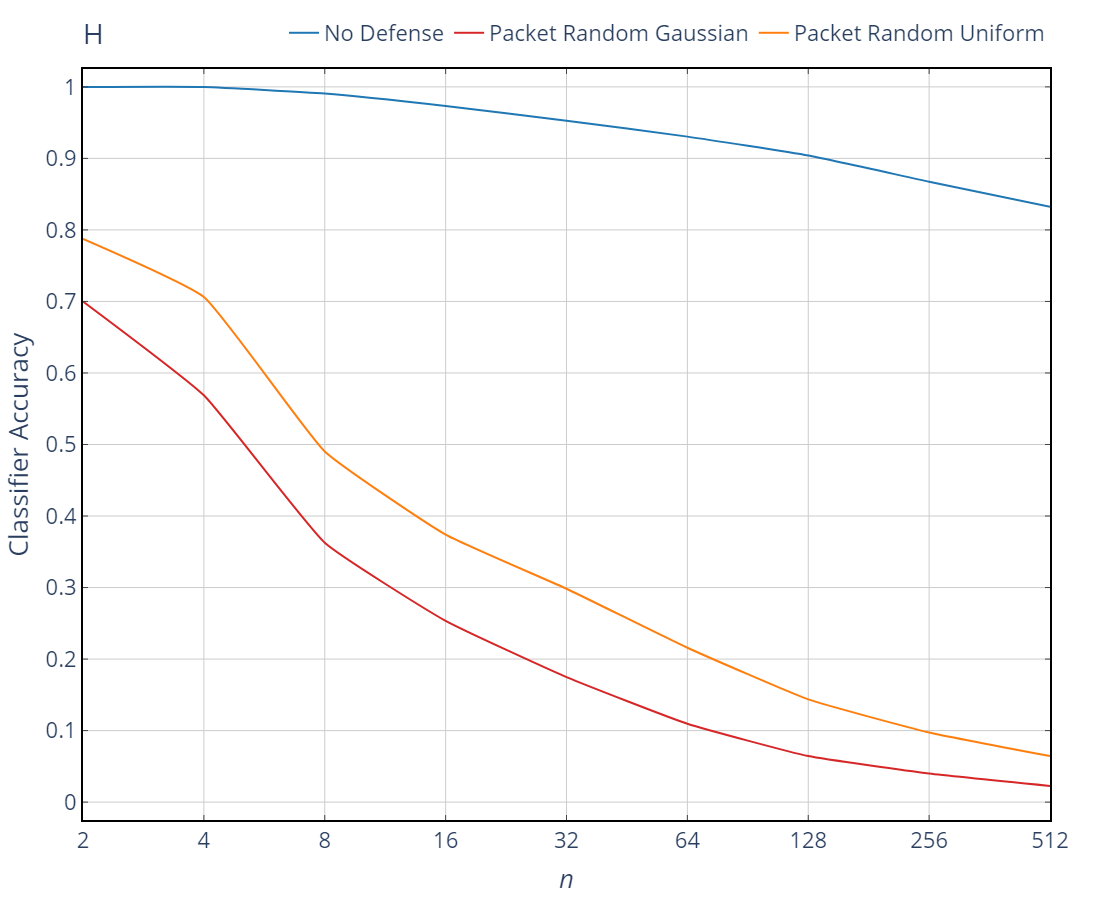
\includegraphics[width=\textwidth]{plots/performance_h_pkt.png}
			\caption{Packet Random Padding}
		\end{subfigure}
		\hfill
		\begin{subfigure}{0.495\textwidth}
			\centering
			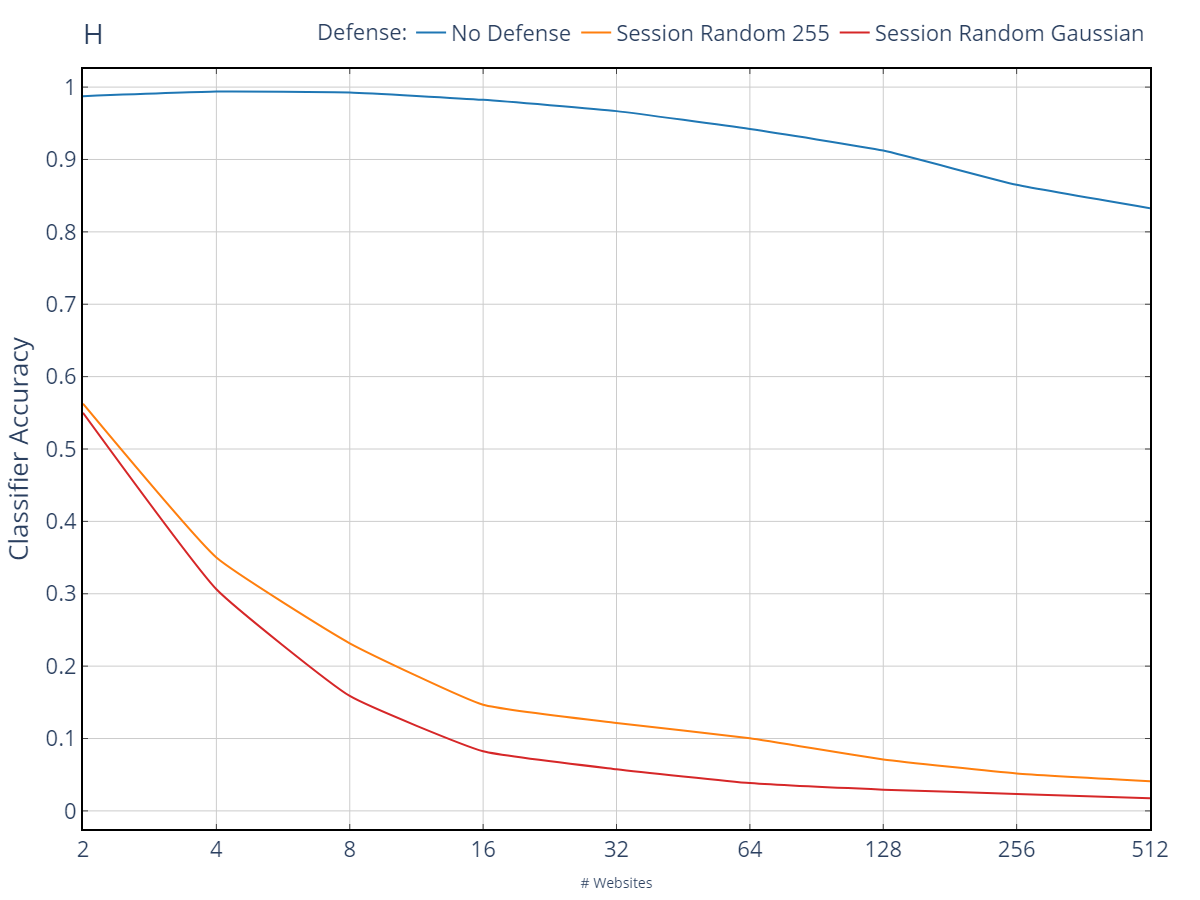
\includegraphics[width=\textwidth]{plots/performance_h_ses.png}
			\caption{Session Random Padding}
		\end{subfigure}
		\caption[Performance of Gaussian padding against the H attack]{Performance of Gaussian padding against the H attack \cite{Herrmann2009} in comparison to uniform padding.}
		\label{fig:h}
	\end{figure}
	\begin{figure}
		\begin{subfigure}{0.495\textwidth}
			\centering
			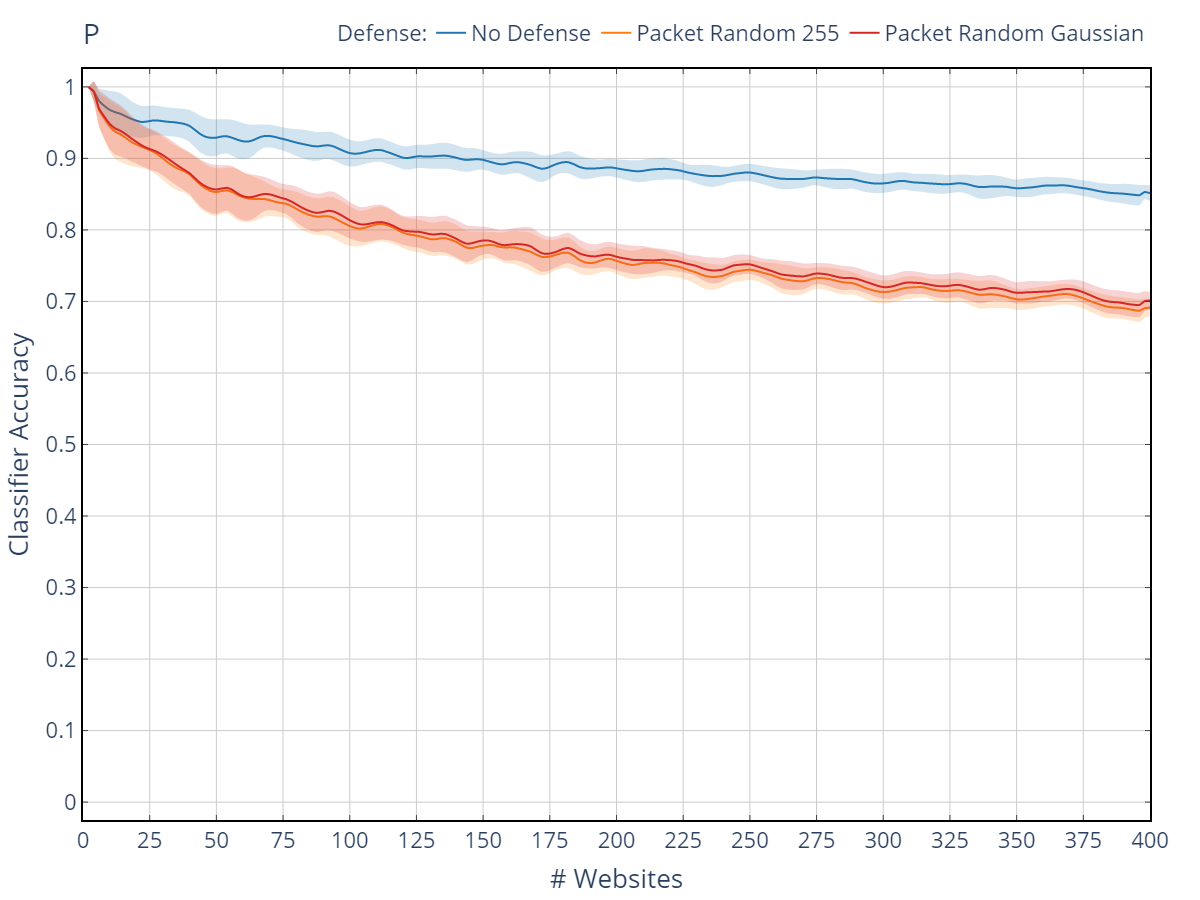
\includegraphics[width=\textwidth]{plots/performance_p_pkt.png}
			\caption{Packet Random Padding}
		\end{subfigure}
       \hfill
		\begin{subfigure}{0.495\textwidth}
			\centering
			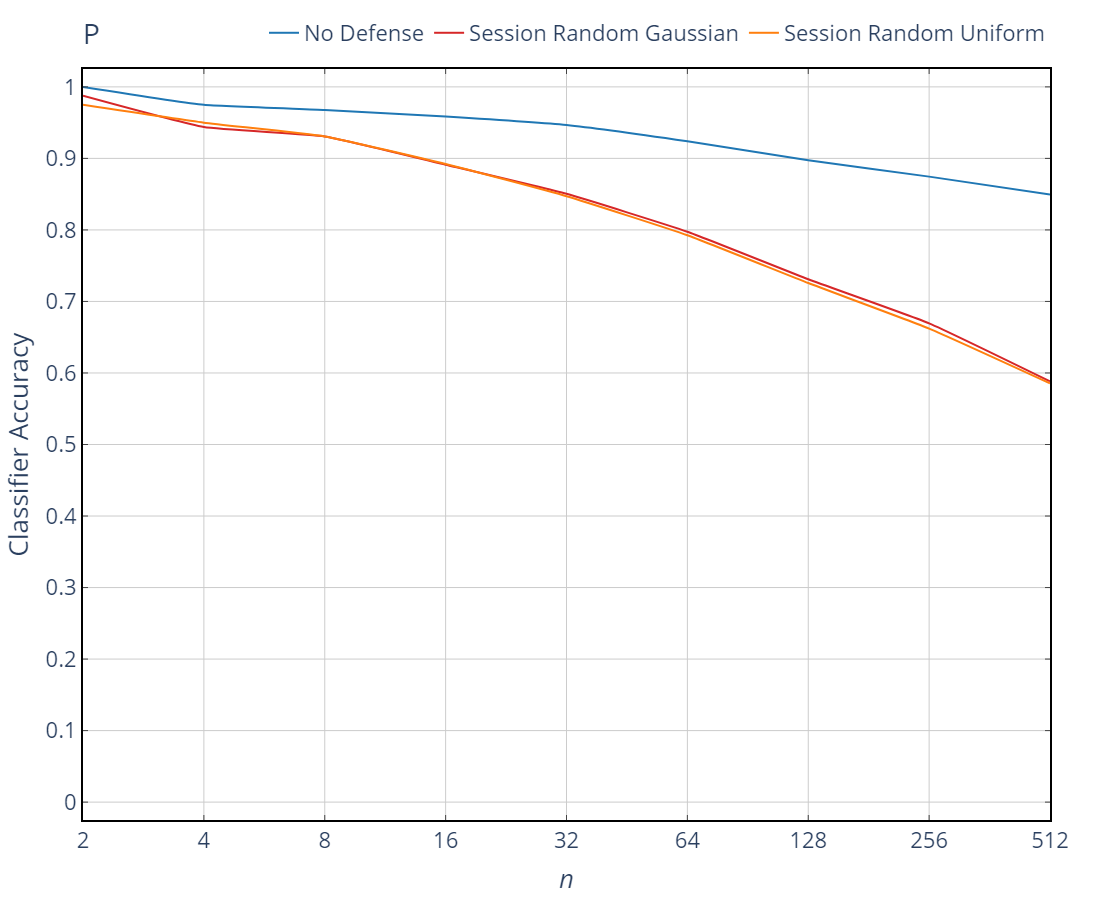
\includegraphics[width=\textwidth]{plots/performance_p_ses.png}
			\caption{Session Random Padding}
		\end{subfigure}
		\caption[Performance of Gaussian padding against the P attack]{Performance of Gaussian padding against the P attack \cite{Panchenko2011} in comparison to uniform padding.}
		\label{fig:p}
	\end{figure}
	\begin{figure}
		\begin{subfigure}{0.495\textwidth}
			\centering
			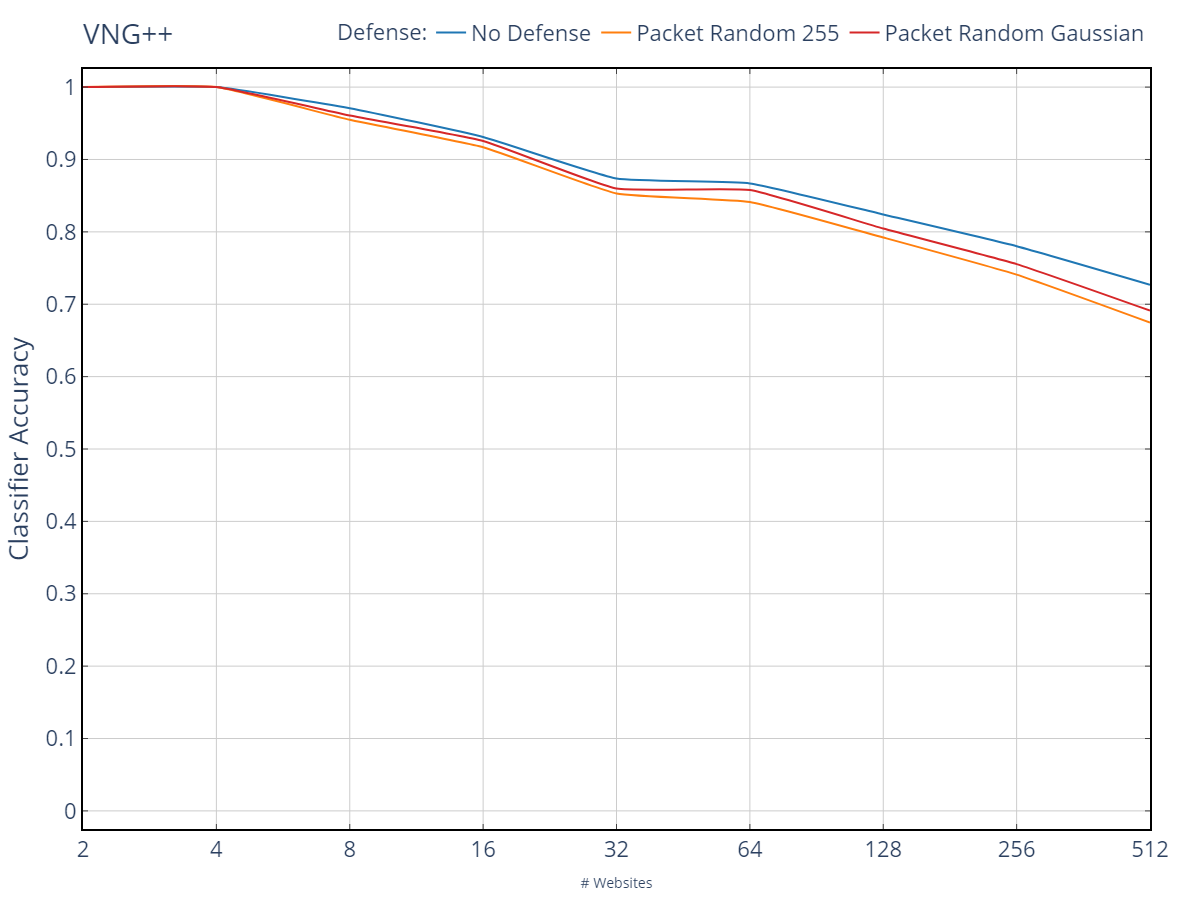
\includegraphics[width=\textwidth]{plots/performance_vng++_pkt.png}
			\caption{Packet Random Padding}
		\end{subfigure}
		\hfill
		\begin{subfigure}{0.495\textwidth}
			\centering
			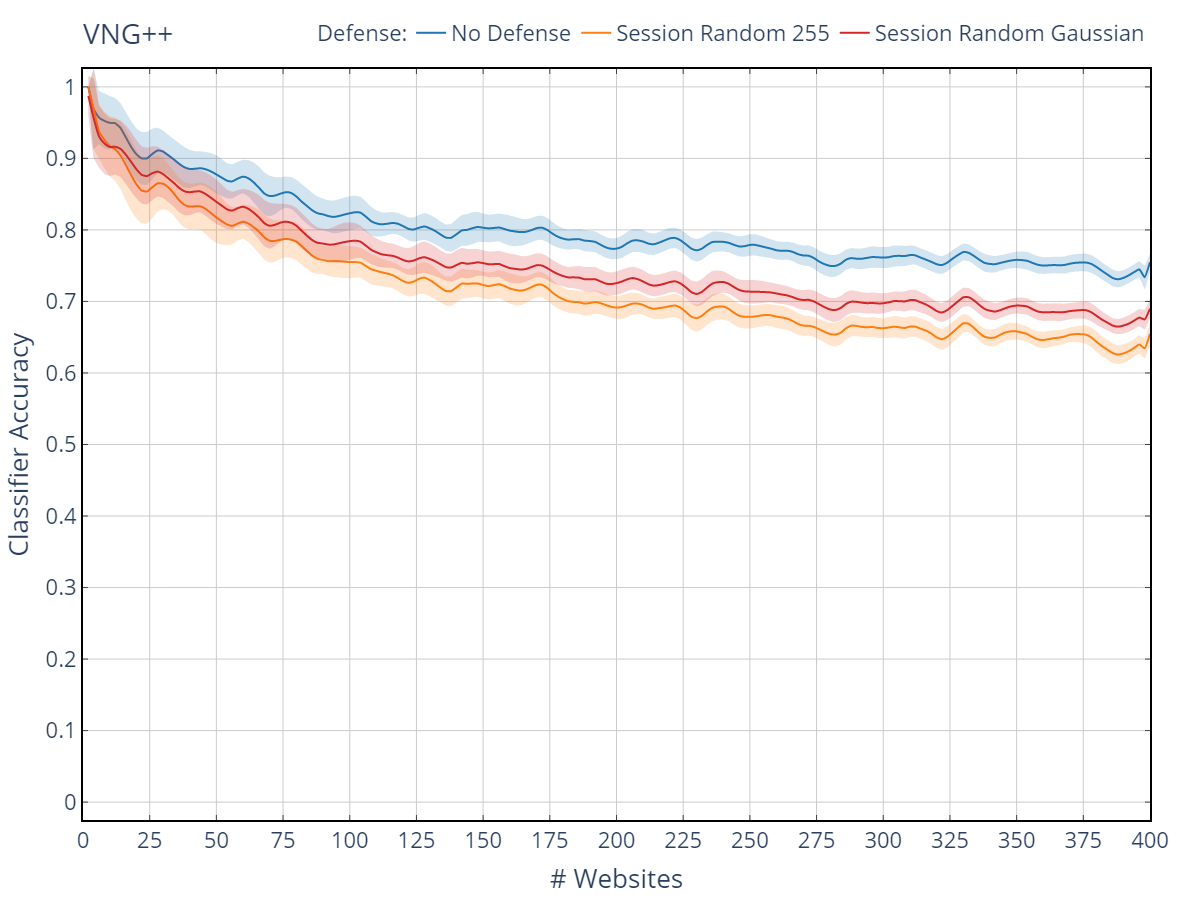
\includegraphics[width=\textwidth]{plots/performance_vng++_ses.png}
			\caption{Session Random Padding}
		\end{subfigure}
		\caption[Performance of Gaussian padding against the VNG++ attack]{Performance of Gaussian padding against the VNG++ attack \cite{Dyer2012} in comparison to uniform padding.}
		\label{fig:vng++}
	\end{figure}
	% TODO Add CUMUL

	\subsection{Bandwidth Overhead}
	
	For all defenses in question, data on the bandwidth overhead was collected. Therefore, each defense was evaluated 50 times on 128 randomly chosen websites with 25 traces per website, chosen from a randomly selected offset. The sum of all packet sizes in both directions was calculated before and after applying the padding. The results of this calculation are presented in Table \ref{tbl:overhead}. Additionally, Figure \ref{fig:overhead} gives an overview about the distribution of bandwidth overhead.
	
	All in all, Gaussian padding does not account for considerably higher bandwidth overhead. In the packet random scheme, the difference of 0.04\% is significant (significance level of 99\%), whereas the session random padding methods do not show a significant difference.
	
	\begin{table}
		\centering
		\begin{tabular}{lcc}
			\toprule \textbf{Scheme} & \textbf{Distribution} & \breakable{\textbf{Bandwidth}\\ \textbf{Overhead (\%)}} \\			
			\midrule Packet Random & Uniform & $16.69 \pm 1.31$\\
			 & Gaussian & $16.73 \pm 1.31$ \\ \addlinespace
			Session Random & Uniform & $16.75 \pm 1.29$ \\
			& Gaussian & $16.74 \pm 1.36$ \\
			\bottomrule
		\end{tabular}
		\caption{Average bandwidth overhead of uniform and Gaussian padding in the packet random and session random schemes}
		\label{tbl:overhead}
	\end{table}

	\begin{figure}
		\centering
		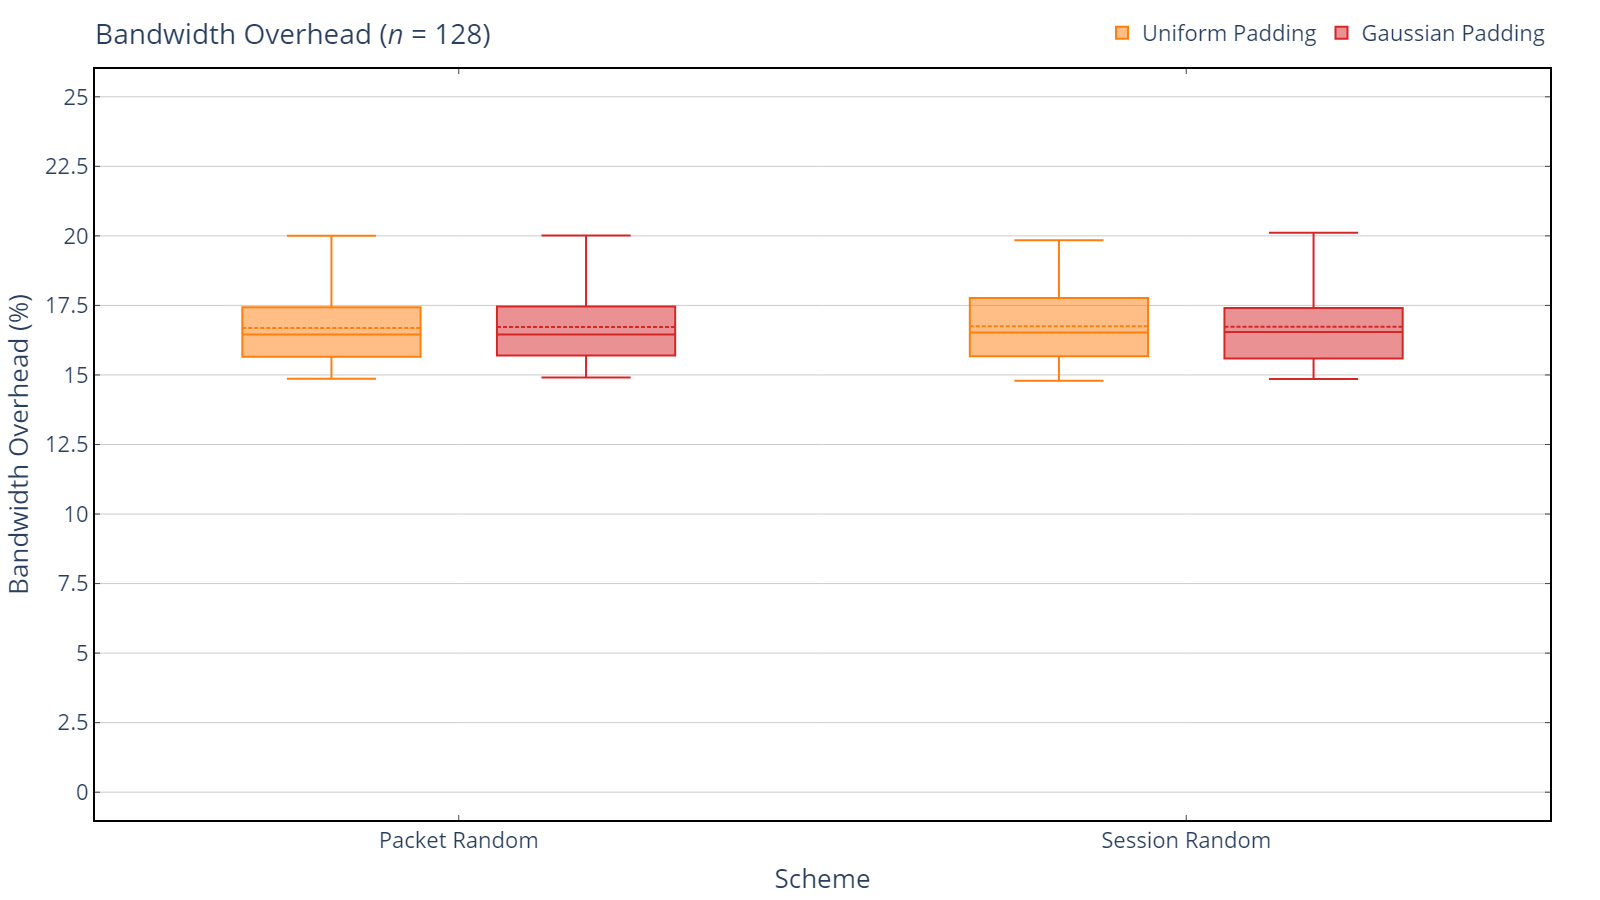
\includegraphics[width=\textwidth]{plots/overhead.png}
		\caption[Bandwidth overhead of uniform and Gaussian padding in the packet random and session random schemes]{Bandwidth overhead of uniform and Gaussian padding in the packet random and session random schemes. The mean is marked as a dashed line.}
		\label{fig:overhead}
	\end{figure}

	\subsection{Significance Testing}
	\label{results:sig_score}
	
	To calculate the significance of the previously mentioned observations, the results from the second experiment were used. For each pair of attack and defense, the classification accuracy was measured 50 times. Figure \ref{fig:performance_dist} displays a distribution plot of the results. Subsequently, the measured accuracy values were used to conduct a paired t-test on the differences of the average accuracy for uniform and Gaussian padding. The null hypothesis was that the actual means of the classifier accuracy were equal for uniform and Gaussian padding. Table \ref{tbl:sig_score} shows the results of the test.
	
	Overall, the Gaussian padding methods perform significantly better than uniform padding for a significance level of 99\% against both, the LL and H attacks. In contrast, for the VNG++ and CUMUL attacks in the packet-random scheme, uniform padding performs significantly better than Gaussian padding for the same significance level. The P attack yields no significant difference against the packet-random scheme, while the same goes for the CUMUL attack against the session-random scheme with a significance level of 99\%. However, when lowering the significance level to 95\%, uniform padding performs significantly better than Gaussian padding against the CUMUL attack. Using the session random scheme against the P and VNG++ attack, uniform padding performs significantly better than Gaussian padding.
		
	\begin{figure}
		\begin{subfigure}{0.495\textwidth}
			\centering
			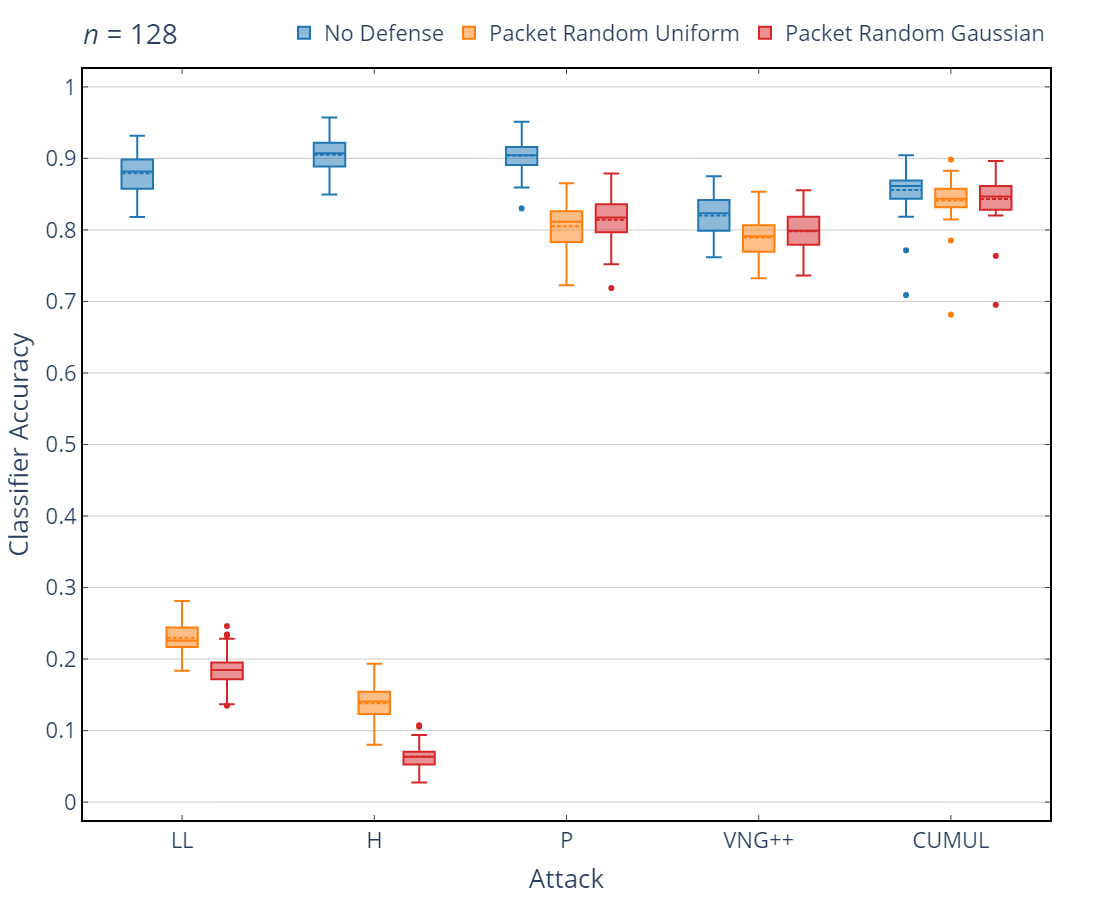
\includegraphics[width=\textwidth]{plots/significance_pkt.png}
			\caption{Packet Random Padding}
		\end{subfigure}
		\hfill
		\begin{subfigure}{0.495\textwidth}
			\centering
			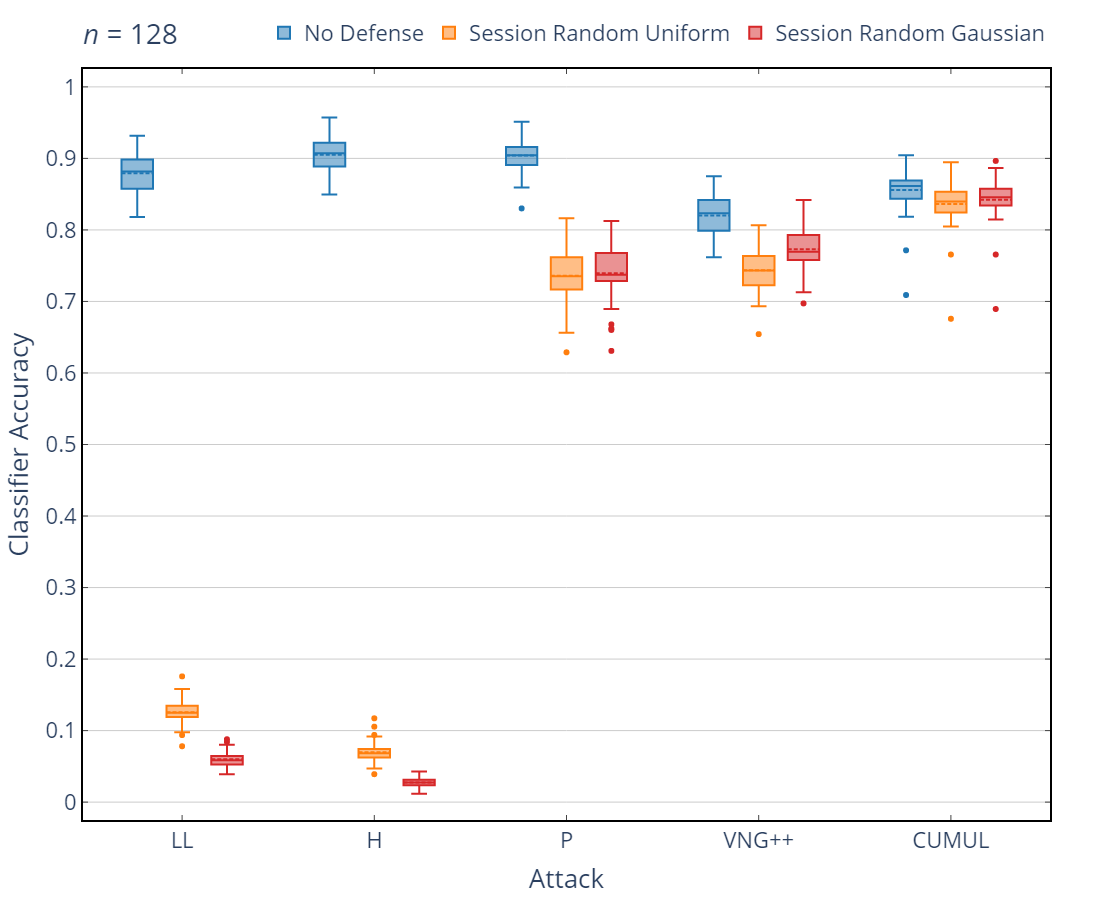
\includegraphics[width=\textwidth]{plots/significance_ses.png}
			\caption{Session Random Padding}
		\end{subfigure}
		\caption[Distribution of classifier accuracy against Gaussian Padding on 128 Websites]{Distribution of classifier accuracy against Gaussian Padding on 128 Websites in comparison with uniform padding}
		\label{fig:performance_dist}
	\end{figure}

	\begin{table}
		\centering
		\small
		% TODO Add new performance values
		\begin{tabular}{llcccc}
			\toprule \textbf{Attack} & \textbf{Scheme} & $\mathbf{\mu^*_{u}}$ \textbf{(\%)} & $\mathbf{\mu^*_{g}}$  \textbf{(\%)} & $\mathbf{t}$ & $\mathbf{\alpha}$ \\
			\midrule LL & Packet & $23.39 \pm 2.71$ & $\mathbf{18.54 \pm 2.73}$ & $15.95$ & $0.000$\\
			 & Session & $13.44 \pm 1.74$ & $\mathbf{6.15 \pm 1.19}$ & $27.19$ &  $0.000$\\ \addlinespace
			H & Packet & $14.75 \pm 2.54$ & $\mathbf{6.75 \pm 1.81}$ & $30.52$ & $0.000$ \\
			& Session & $7.26 \pm 1.42$ & $\mathbf{2.83 \pm 0.83}$ & $19.49$ & $0.000$ \\ \addlinespace
			P & Packet & $80.67 \pm 3.19$ & $80.86 \pm 3.07$ & $-0.98$ & $0.833$ \\
			& Session & $\mathbf{73.05 \pm 3.54}$ & $73.83 \pm 3.57$ & $-2.69$ & $0.995$ \\ \addlinespace
			VNG++ & Packet & $\mathbf{80.06 \pm 2.99}$ & $80.98 \pm 2.84$ & $-3.97$ & $1.000$ \\
			& Session & $\mathbf{75.52 \pm 3.18}$ & $78.23 \pm 3.20$ & $-11.18$ & $1.000$ \\ \addlinespace
			CUMUL & Packet & $\mathbf{83.83\pm 2.82}$ & $84.38 \pm 2.67$ & $-4.72$ & $1.000$\\
			& Session & $83.53 \pm 2.94$ & $83.91 \pm 2.85$ & $-2.63$ & $0.994$ \\
			\bottomrule
		\end{tabular}
		\caption[Significance Testing of padding performance for $n = 128$]{Significance Testing of padding performance for $n = 128$. $\mu^*_u$ and $\mu^*_g$ denote the observed average classifier accuracy for uniform and Gaussian padding, respectively. $\alpha$ denotes the probability of a Type I error when rejecting the null hypothesis that the real mean $\mu_g$ is greater than or equal to $\mu_u$. Significantly better values wrt. a significance level of 99\% are printed bold. }
		\label{tbl:sig_score}
	\end{table}

	\section{Estimated Security Bounds}
	\label{security_bounds}
	
	Table \ref{tbl:error_bound} shows the results of error bound estimation in the closed world and open world scenarios for all combinations of attack and defense. The estimated bounds differ largely between defenses, while some are very close to the observed classifier error. In particular, the results for the packet random schemes in the closed world scenario are closest to the empirical classifier error of the LL and H attacks. In contrast, the error bound of the Session Random Uniform defense is really far from the classifier error of those attacks, reaching over 80\% difference for the H attack. 
	
	\paragraph{Closed World Scenario} The error bounds in the closed world scenario display a similar behavior as the classifier accuracy, showing Gaussian padding schemes as superior against the LL and H attacks, while uniform schemes have an advantage against VNG++ and CUMUL. Different from the empirical classifier error, however, is the error bound of the P attack, which reaches the highest value for Session Random Gaussian padding. Notably, the error bounds of the CUMUL attack are all very close to each other, laying within a range of 0.5\%, repeating the measurements of classifier performance that also were very close.
	
	\paragraph{Open World (One-vs-All) Scenario} As opposed to the closed world, the one-vs-all scenario results in considerably lower error bounds throughout all measurements. The general relationship between the attacks and defenses, however, is mostly the same, with Gaussian padding winning against LL and H and uniform padding leading to better results against VNG++ and CUMUL. For the P attack, the packet random schemes do not differ while Session Random Gaussian wins over Session Random Uniform. Generally speaking, in the open world scenario, the error bound differences are relatively small within the same attack, laying all within a range of less than 1.5\% for P, VNG++ and CUMUL when applying any defense. For the CUMUL attack, the difference between using no defense and the best-performing defense (Session Random Uniform) is even only 0.18\%. In constrast to that, the LL and H attacks are showing larger differences between error bounds for different defenses.

	\begin{table}
		% TODO New values and make all numbers math mode
		\centering
		\small
		\begin{tabular}{llcccc}
			\toprule 
			& & \multicolumn{2}{c}{\textbf{Closed World}} & \multicolumn{2}{c}{\textbf{Open World (One vs All)}} \\
			\textbf{Attack} & \textbf{Defense} & $\mathbf{\widehat{R}^*}$ \textbf{(\%)} & $\mathbf{\varepsilon}\textbf{-Privacy}$ & $\mathbf{\widehat{R}^*}$ \textbf{(\%)} & $\mathbf{\varepsilon}\textbf{-Privacy}$ \\
			\midrule
			\textbf{LL} & None & $4.76 \pm 1.55$ & 0.05 & $1.47\pm 0.20$ & 0.03 \\
			 & Packet Random Uniform & $37.09 \pm 2.12$ & 0.37 & $6.09\pm 0.62$ & 0.12 \\
			 & Packet Random Gaussian & $\mathbf{55.65 \pm 2.48}$ & \textbf{0.56} & $\mathbf{16.86\pm 1.58}$ & \textbf{0.34} \\
			 & Session Random Uniform & $15.42 \pm 1.77$ & 0.16 & $5.81\pm 0.38$ & 0.12 \\
			 & Session Random Gaussian & $41.01 \pm 1.40$ & 0.41 & $13.26\pm 0.72$ & 0.27 \\ \addlinespace
			 
		    \textbf{H} & None & $3.69 \pm 1.50$ & 0.04 & $1.42\pm 0.14$ & 0.03 \\
			 & Packet Random Uniform & $56.51 \pm 2.04$ & 0.57 & $14.97\pm 1.26$ & 0.30 \\
			 & Packet Random Gaussian & $\mathbf{68.21 \pm 2.16}$ & \textbf{0.69} & $22.37\pm 2.65$ & 0.45 \\
			 & Session Random Uniform & $9.44 \pm 1.52$ & 0.10 & $12.90\pm 0.32$ & 0.26 \\
			 & Session Random Gaussian & $39.98 \pm 0.91$ & 0.40 & $\mathbf{29.84\pm 0.82}$ & \textbf{0.60} \\ \addlinespace
			 
			\textbf{P} & None & $5.11 \pm 1.54$ & 0.05 & $1.57 \pm 0.17$ & 0.01 \\
			 & Packet Random Uniform & $10.76 \pm 1.97$ & 0.11 & $2.06 \pm 0.24$ & 0.04 \\
			 & Packet Random Gaussian & $10.35 \pm 1.97$ & 0.10 & $2.06 \pm 0.26$ & 0.04 \\
			 & Session Random Uniform & $14.26 \pm 1.84$ & 0.14 & $3.04 \pm 0.33$ & 0.06 \\
			 & Session Random Gaussian & $\mathbf{24.57 \pm 1.97}$ & \textbf{0.25} & $\mathbf{3.41 \pm 0.36}$ & \textbf{0.07} \\ \addlinespace
			 
			\textbf{VNG++} & None & $10.38 \pm 1.75$ & 0.10 & $2.46 \pm 0.33$ & 0.05 \\
			 & Packet Random Uniform & $13.33\pm 1.87$ & 0.13 & $2.59 \pm 0.32$ & 0.05 \\
			 & Packet Random Gaussian & $12.39 \pm 1.80$ & 0.13 & $2.54 \pm 0.33$ & 0.05 \\
			 & Session Random Uniform & $\mathbf{17.22 \pm 1.98}$ & \textbf{0.17} & $\mathbf{3.13 \pm 0.35}$ & \textbf{0.06} \\
			 & Session Random Gaussian & $14.94\pm 1.86$ & 0.15 & $2.82 \pm 0.31$ & \textbf{0.06} \\ \addlinespace
			 
			\textbf{CUMUL} & None & $7.30 \pm 1.56$  & 0.07 & $2.40\pm 0.32$ & 0.05 \\
			 & Packet Random Uniform & $8.49 \pm 1.72$ & \textbf{0.09} & $2.49 \pm 0.32$ & 0.05 \\
			 & Packet Random Gaussian & $8.08 \pm 1.69$ & 0.08 & $2.47\pm 0.31$ & 0.05 \\
			 & Session Random Uniform & $\mathbf{8.52 \pm 1.66}$ & \textbf{0.09} & $\mathbf{2.58 \pm 0.32}$ & 0.05 \\
			 & Session Random Gaussian & $8.15 \pm 1.66$ & 0.08 & $2.52\pm 0.36$ & 0.05 \\
			\bottomrule
		\end{tabular}
		\caption[Error bound results for all attacks and defenses]{Error bound results for all attacks and defenses, showing the average error bound and standard deviation. The best value for each attack is printed in bold.}
		\label{tbl:error_bound}
	\end{table}

	\begin{figure}
		\begin{subfigure}{0.495\textwidth}
			\centering
			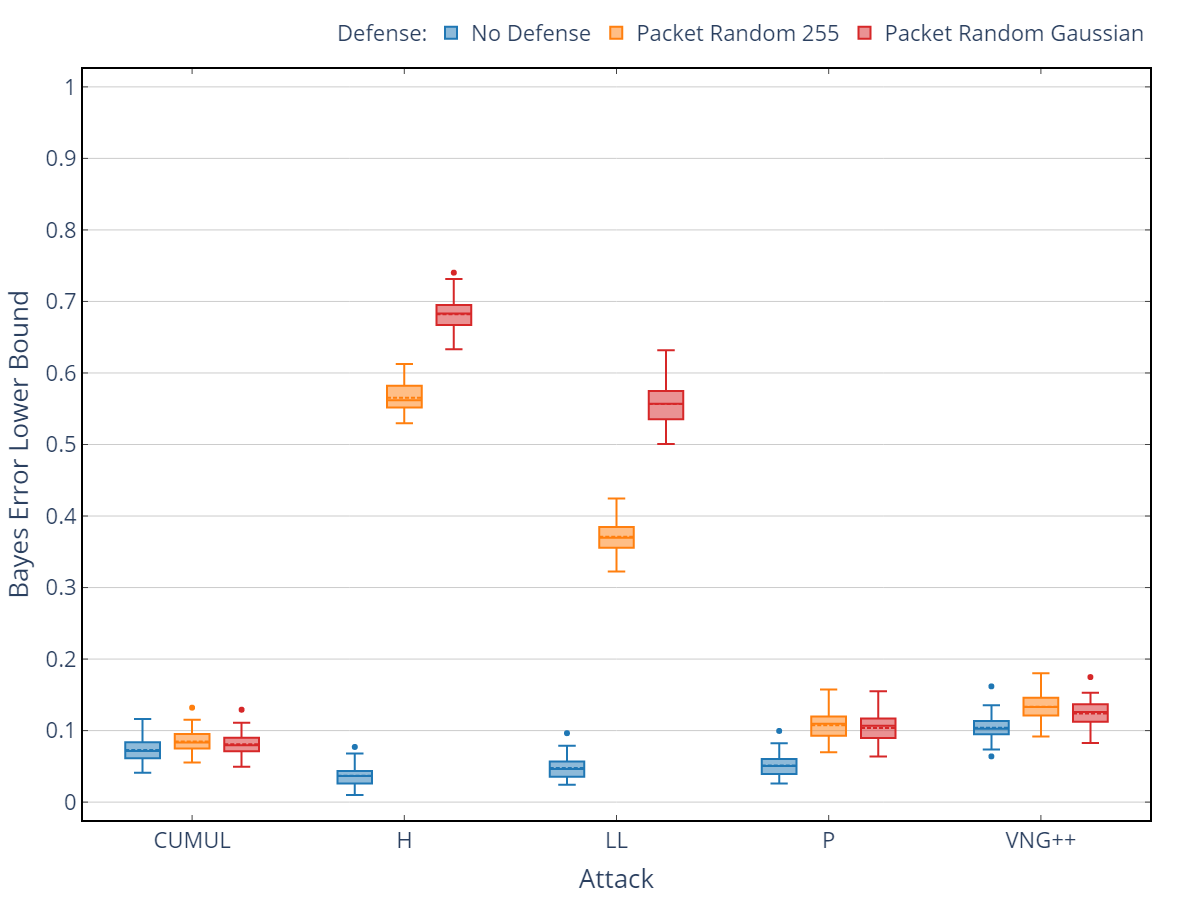
\includegraphics[width=\textwidth]{plots/bounds_cw_pkt.png}
			\caption{Packet Random Padding\\Closed World}
		\end{subfigure}
		\hfill
		\begin{subfigure}{0.495\textwidth}
			\centering
			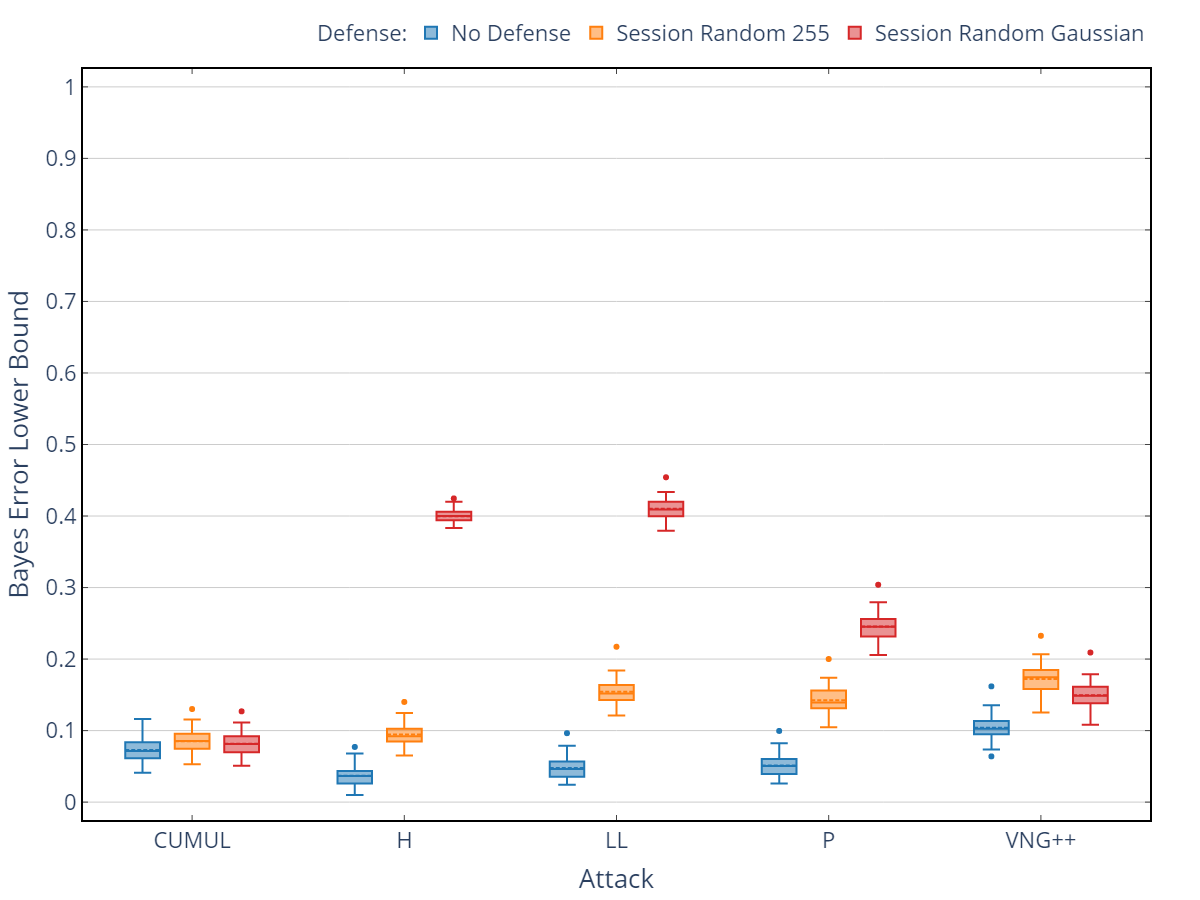
\includegraphics[width=\textwidth]{plots/bounds_cw_ses.png}
			\caption{Session Random Padding\\Closed World}
		\end{subfigure}
		\caption[Lower Bounds for the Bayes Error in the closed world scenario]{Lower Bounds for the Bayes Error in the closed world scenario using Gaussian Padding on 100 Websites in comparison with uniform padding}
		\label{fig:bound_cw}
	\end{figure}
	\begin{figure}
		\begin{subfigure}{0.495\textwidth}
			\centering
			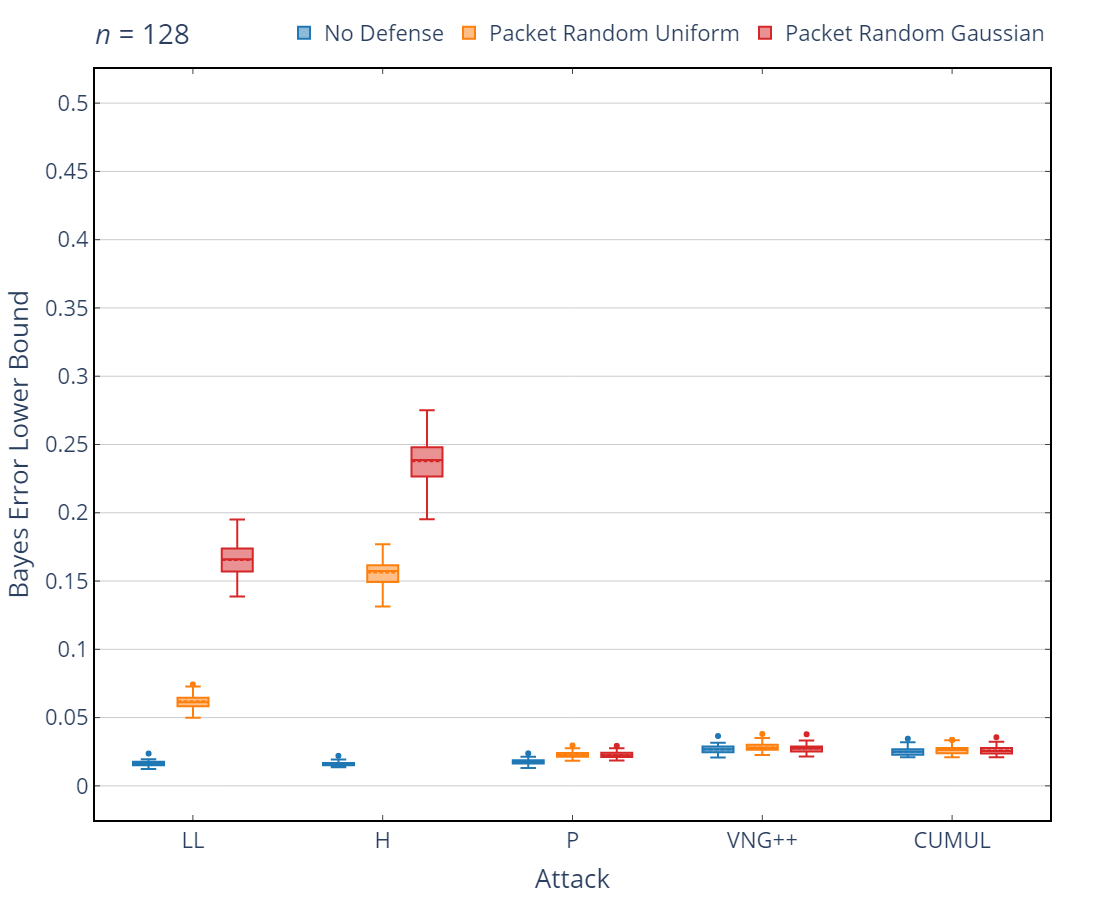
\includegraphics[width=\textwidth]{plots/bounds_ow_pkt.png}
			\caption{Packet Random Padding\\Open World}
		\end{subfigure}
		\hfill
		\begin{subfigure}{0.495\textwidth}
			\centering
			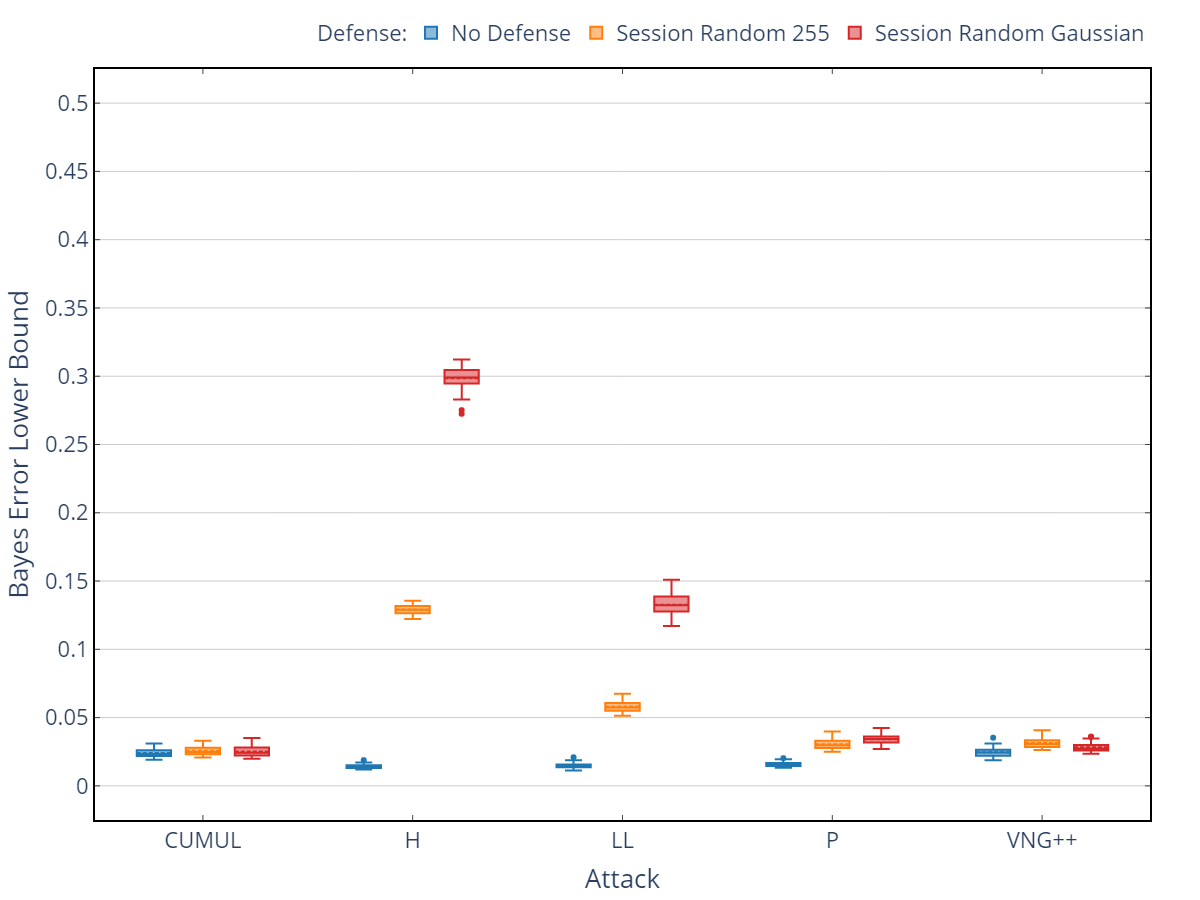
\includegraphics[width=\textwidth]{plots/bounds_ow_ses.png}
			\caption{Session Random Padding\\Open World}
		\end{subfigure}
		\caption[Lower Bounds for the Bayes Error in the open world scenario]{Lower Bounds for the Bayes Error in the open world scenario using Gaussian Padding on 100 Websites in comparison with uniform padding}
		\label{fig:bound_ow}
	\end{figure}

	\subsection{Significance Testing}
	
	Analogous to the procedure described in Section \ref{results:sig_score}, a significance test was applied to the calculated error bounds. The null hypothesis was that the mean error bounds for uniform and Gaussian padding are equal. The test was carried out separately for the closed world and open world scenarios, respectively.
	
	\paragraph{Closed World Scenario} Table \ref{tbl:sig_bound_cw} gives the results of significance testing in the closed world scenario. Similarly to when comparing classifier accuracy, Gaussian padding achieves significantly better error bounds against the LL and H attacks. Additionally, the Session Random Gaussian schema is significantly better than Session Random Uniform against P. For VNG++ and CUMUL, the advantage of uniform padding is significant in both schemes, as well as for the packet random scheme against the P attack.
	
	\begin{table}
		\centering
		\small
		% TODO Add new error bound values
		\begin{tabular}{llcccc}
			\toprule \textbf{Attack} & \textbf{Scheme} & $\mathbf{\widehat{R}^*_u}$ \textbf{(\%)} & $\mathbf{\widehat{R}^*_g}$  \textbf{(\%)} & $\mathbf{t}$ & $\mathbf{\alpha}$ \\
			\midrule LL & Packet & $37.09 \pm 2.12$ & $\mathbf{55.65 \pm 2.48}$ & $-58.30$ & $0.000$\\
			& Session & $15.42 \pm 1.78$ & $\mathbf{41.01 \pm 1.40}$ & $-151.47$ &  $0.000$\\ \addlinespace
			H & Packet & $56.525 \pm 2.04$ & $\mathbf{68.21 \pm 2.16}$ & $-36.45$ & $0.000$ \\
			& Session & $9.44 \pm 1.52$ & $\mathbf{39.98 \pm 0.91}$ & $-223.88$ & $0.000$ \\ \addlinespace
			P & Packet & $\mathbf{10.76 \pm 1.97}$ & $10.35 \pm 1.97$ & $11.51$ & $1.000$ \\
			& Session & $14.26 \pm 1.84$ & $\mathbf{24.57 \pm 1.97}$ & $-63.20$ & $0.000$ \\ \addlinespace
			VNG++ & Packet & $\mathbf{13.33 \pm 1.87}$ & $12.39 \pm 1.80$ & $21.32$ & $1.000$ \\
			& Session & $\mathbf{17.22 \pm 1.98}$ & $14.94 \pm 1.86$ & $36.90$ & $1.000$ \\ \addlinespace
			CUMUL & Packet & $\mathbf{8.49\pm 1.72}$ & $8.08 \pm 1.69$ & $15.36$ & $1.000$\\
			& Session & $\mathbf{8.52 \pm 1.66}$ & $8.15 \pm 1.66$ & $16.28$ & $1.000$ \\
			\bottomrule
		\end{tabular}
		\caption[Significance Testing of error bounds in the closed world scenario]{Significance Testing of error bounds in the closed world scenario. $\widehat{R}^*_u$ and $\widehat{R}^*_g$ denote the observed average error bound for uniform and Gaussian padding, respectively. $\alpha$ denotes the probability of a Type I error when rejecting the null hypothesis that the real mean $\widehat{R}_g$ is less than or equal to $\widehat{R}_u$. Significantly better values wrt. a significance level of 99\% are printed bold. }
		\label{tbl:sig_bound_cw}
	\end{table}

	\paragraph{Open World (One-vs-All) Scenario} The significance results for the open-world scenario are presented in Table \ref{tbl:sig_bound_ow}. The only combinations not yielding a significant difference were the P and CUMUL attacks against the packet random schemes, where no padding distribution brought any advantage. For LL and H, Gaussian padding had a significantly better error bound in both padding schemes, which also applies to the session random scheme and the P attack. The remaining cases, namely the VNG++ attack in both schemes, and the CUMUL attack in the session random scheme, uniform padding yielded a significantly higher bound, although not a large difference.
	
	\begin{table}
		\centering
		\small
		% TODO Add new error bound values
		\begin{tabular}{llcccc}
			\toprule \textbf{Attack} & \textbf{Scheme} & $\mathbf{\widehat{R}^*_u}$ \textbf{(\%)} & $\mathbf{\widehat{R}^*_g}$  \textbf{(\%)} & $\mathbf{t}$ & $\mathbf{\alpha}$ \\
			\midrule LL & Packet & $6.09 \pm 0.62$ & $\mathbf{16.86 \pm 1.58}$ & $-57.08$ & $0.000$\\
			& Session & $5.81 \pm 0.38$ & $\mathbf{13.26 \pm 0.72}$ & $-87.46$ &  $0.000$\\ \addlinespace
			H & Packet & $14.97 \pm 1.26$ & $\mathbf{22.37 \pm 2.65}$ & $-27.94$ & $0.000$ \\
			& Session & $12.90 \pm 0.32$ & $\mathbf{29.84 \pm 0.82}$ & $-153.31$ & $0.000$ \\ \addlinespace
			P & Packet & $2.06 \pm 0.24$ & $2.06 \pm 0.26$ & $0.13$ & $0.550$ \\
			& Session & $3.04 \pm 0.33$ & $\mathbf{3.41 \pm 0.36}$ & $-11.74$ & $0.000$ \\ \addlinespace
			VNG++ & Packet & $\mathbf{2.59 \pm 0.32}$ & $2.54 \pm 0.33$ & $3.15$ & $0.999$ \\
			& Session & $\mathbf{3.13 \pm 0.35}$ & $2.82 \pm 0.31$ & $15.84$ & $1.000$ \\ \addlinespace
			CUMUL & Packet & $2.49\pm 0.32$ & $2.47 \pm 0.31$ & $1.70$ & $0.952$\\
			& Session & $\mathbf{2.58 \pm 0.32}$ & $2.52 \pm 0.36$ & $3.51$ & $1.000$ \\
			\bottomrule
		\end{tabular}
		\caption[Significance Testing of error bounds in the open world scenario]{Significance Testing of error bounds in the open world (one-vs-all) scenario. $\widehat{R}^*_u$ and $\widehat{R}^*_g$ denote the observed average error bound for uniform and Gaussian padding, respectively. $\alpha$ denotes the probability of a Type I error when rejecting the null hypothesis that the real mean $\widehat{R}_g$ is less than or equal to $\widehat{R}_u$. Significantly better values wrt. a significance level of 99\% are printed bold. }
		\label{tbl:sig_bound_ow}
	\end{table}

	\chapter{Discussion}
	\label{discussion}
	\IMRADlabel{discussion}

	When surveying the results from the previous section, one major thing to notice is that attacks seem to fall into two categories with regard to their performance against uniform and Gaussian padding. On the one hand, there are the LL and H attack, against which both padding schemes are largely effective, while on the other hand, the VNG++ and CUMUL attacks do not show particular vulnerability to these defenses. The P attack is located between those extreme examples, being more vulnerable to these padding schemes than VNG++ and CUMUL, but still displaying considerably better robustness than LL and H. This seems to suggest, that attacks which use the histogram of packet sizes for features (LL and H) are vulnerable to the randomized padding schemes, while those relying only on coarse grained features (VNG++ and CUMUL) are robust against them. P embodies the special case using both, the packet histogram \textit{and} coarse-grained features, thus explaining the moderate vulnerability and robustness.
	
	Furthermore, a notable difference between attacks with coarse-grained features and histograms is the relation between Gaussian and uniform padding. For those attacks with fine-grained histogram features, Gaussian padding performs significantly better, while for most coarse-grained attack, uniform padding had a significant advantage, if any. This shows that the Gaussian distribution is well-suited to disguise identifying patterns in the packet histograms of websites, explaining the efficacy against the LL and H attacks. However, considering modern attacks that are using mostly coarse-grained features (cf. \cite{Dyer2012,Wang2014,Panchenko2016,Hayes2016}), the effect of applying the Gaussian distribution for padding must be assumed rather small. Taking into context the fact that uniform padding also performed poorly against the CUMUL attack, this points to a general ineffectiveness of simple randomized padding schemes against modern attacks. This also aligns with the previous findings of Dyer et al., who noted that padding schemes are insufficient to reliably hide coarse-grained features of website traces \cite{Dyer2012}.
	
	Going further, the reported advantage of the session over packet random padding schemes may be explained by a simple statistical effect: When using packet random padding on a sufficiently long trace, the distribution of mean padding length converges to a normal distribution having the same expected value as the padding distribution, due to the \textit{Central Limit Theorem} \cite{Fischer2010}. This leads to the effect of randomness already averaging out to a certain degree over each trace, resulting in less variation. However, this isn't the case for session random padding, where the mean padding length for a trace is simply the value drawn from the padding distribution. In consequence, the feature extraction algorithm has to deal with a higher variance in trace data. This is supported by the fact that session random padding has a particular advantage against attacks that do not reduce the trace data's variance much in the feature extraction such as LL, H and P (partially), as can be clearly seen in Table \ref{tbl:sig_score}. On the other hand, the CUMUL attack doesn't show considerable advantage for session random padding, suggesting that the CUMUL feature set is well suited to lower sample variance among the traces of a website. Taking this argument even further, it can be concluded that no packet random padding scheme is likely to perform well against a good selection of coarse-grained features, as the combination of multiple packets into a single feature leads to the randomness averaging out, the effect getting stronger the more packets are combined. In consequence, the mean padding length within a single feature converges against the expected value of the padding distribution, yielding features that are very similar to those of the undefended trace, each feature offset by some value that is normally distributed. This effect keeps the features still easily distinguishable, being only a translated version of the original undefended features, where the translation is likely to be similar for different traces. While this argument can't be directly applied to session random padding, the fact that session random padding expands a point in the feature space to a contiguous subspace (also translating features, but by different amounts for each trace), may serve as a hint that session random padding can blur the lines of a website in the feature space but still keeps its data compact, which aids classification.
	
	Although Gaussian padding doesn't perform well against modern attacks, it represents a very efficient countermeasure for website fingerprinting, having less than 16.7\% of bandwidth overhead and no time overhead. This is a good value compared to other defenses, an overview of which is shown in Table \ref{tbl:overhead_comp}. Also, as compared to uniform padding, Gaussian padding achieves significantly higher performance with a negligible increase in bandwidth overhead against LL and H. However, this must  be set in relation to the bad performance against modern attacks, where a user of anonymization services might prefer to better hide his browsing behavior over having the least overhead possible. From this point of view, the bandwidth advantage of Gaussian padding doesn't have much value as it fails to reliably defend against a WF adversary.
	
	\begin{table}
		\centering
		\begin{tabular}{lcc}
			\toprule \textbf{Defense} & \breakable{\textbf{Bandwidth}\\\textbf{Overhead (\%)}} & \breakable{\textbf{Time}\\\textbf{Overhead (\%)}} \\
			\midrule
			Packet Random Gaussian & 16.73 & 0.00 \\
			Session Random Gaussian & 16.74 & 0.00 \\
			Decoy Pages & 134.4${}^*$ & 59.0${}^*$ \\
			BuFLO & 110.1${}^*$ & 79.1${}^*$ \\
			Tamaraw & 257.6${}^*$ & 341.4${}^*$ \\
			CS-BuFLO & 67.2${}^*$ & 575.6${}^*$ \\
			\bottomrule
		\end{tabular}
	    \caption[Overhead of several recent WF defenses compared to Gaussian padding]{Overhead of several recent WF defenses compared to Gaussian padding.\\{*} = Data from Cherubin's evaluations \cite{Cherubin2017}}
    	\label{tbl:overhead_comp}
	\end{table}
	
	Looking at the results of the error bound analysis, the fact that they mirror the greater patterns of attack performance evaluation is expected. However, there are differences in the details, including large deviations from the actual classifier error, such as in the case of Session Random Uniform padding against the LL and H attacks. This confirms the statement of Cherubin, that a good convergence rate for the error bound estimate can't be guaranteed \cite{Cherubin2017}. It could possible also be a hint that the LL and H classifiers aren't the best possible algorithm for their respective feature set, but considering large gap between the error bound and the empirical error this is probably not the only explanation. The observation of Dyer et al. that the choice of ML classifier doesn't matter so much as the selection of a good feature set supports this interpretation \cite{Dyer2012}. All in all, the error bounds calculated for all defenses go so far as reinforcing that the randomized padding schemes investigated here aren't suitable to reliably thwart attacks that use modern, coarse-grained feature sets. Moreover, the results in the one-vs-all scenario are unsatisfying across the board, yielding lower error bounds below 3.5\% for the P, VNG++ and CUMUL attacks. Considering that the open world scenario is harder to defend but closer to possible real world applications of website fingerprinting, e.g. censorship of internet traffic under authoritarian regimes, the research focus has rightfully shifted towards defenses that perform well in this scenario. Due to the results presented here, Gaussian padding can't be considered to belong in this group.

	\chapter{Conclusion}
	\label{conclusion}
	
	In this thesis, Gaussian padding was evaluated as a defense against Website Fingerprinting attacks. Such attacks have become increasingly successful and robust over the last 10 years, leading to classifiers that achieve more than 95\% accuracy when used to uncover which websites a user has visited. Choosing padding lengths from a rounded truncated Gaussian distribution is a strategy that performed provably better than the uniform distribution when used in the context of padding oracle attacks \cite{Degabriele2021}. These results have prompted the investigation about the efficacy of Gaussian padding against a WF adversary. 
	
	To this end, a generic Python framework for the evaluation of WF attacks and defenses was implemented, including a pipeline for the evaluation of classifier accuracy and one for the estimation of lower bounds for the Bayes error following the method of Cherubin \cite{Cherubin2017}. Experiments were run using the real-world trace data set collected by Liberatore and Levine in 2006 \cite{Liberatore2006}. Prior to evaluation, the data set was analyzed and cleaned to increase the overall data quality and reduce noise due to faulty packet traces. Afterward, the attacks LL, H, P, VNG++ and CUMUL were reimplemented using the \texttt{scikit-learn} machine learning toolkit and evaluated against Gaussian and Uniform padding, both using an expected padding length of 128$\,$byte. Additionally, lower bounds for the Bayes error were estimated for both padding distributions in the closed world and the one-vs-all scenario.
	
	The results are showing a significant advantage of the Gaussian distribution for selecting padding lengths over the uniform distribution when trying to defend against attacks that are using a histogram of individual packet's sizes for features. Furthermore, the efficiency of Gaussian padding is higher than that of uniform padding, achieving a better performance than the latter while not increasing the bandwidth overhead considerably. However, both randomized padding schemes display only poor performance against modern attacks with coarse-grained features, such as VNG++ and CUMUL. In those settings, none of the randomized padding schemes displays the ability to reliably hide the website's identifying characteristics. With the increasing focus on coarse-grained features in recent years, both randomized padding defenses must be considered insufficient against current and future website fingerprinting attacks. Moreover, the open-world scenario is becoming the increasingly important focus of WF research, being the mode that is closer to possible real-world applications of the attacks and defenses. During error bound estimation, the padding schemes performed poorly in the open-world scenario, particularly against modern feature sets, further reinforcing the point that randomized padding isn't a sufficient defense against modern real-world WF adversaries.
	
	What remains to be seen is whether Gaussian padding can serve as a complementary measure to increase the performance of another WF defense that does better at diffusing coarse-grained characteristics of packet traces, such as BuFLO and Tamaraw. Furthermore, an application in combination with Decoy Pages may be an interesting course for further studies, with Decoy Pages breaking up coarse-grained patterns and Gaussian padding diffusing fine-grained characteristics. Other open questions include whether the selected mean padding length of 128$\,$byte represents the best trade-off between bandwidth overhead and defense performance, or if there's a distribution that performs even better than the rounded truncated Gaussian for selecting padding lengths. All in all, Gaussian padding has been shown to have favorable properties for use in the context of website fingerprinting, reaching a better performance and higher bandwidth efficiency than uniform padding. However, the version under investigation here seems to be insufficient on its own to defend against modern WF adversaries.

	\pagebreak
	\pagenumbering{roman}
	\setcounter{page}{5}
	\addcontentsline{toc}{chapter}{Bibliography}
	\printbibliography

	\cleardoublepage
	\phantomsection
	\addcontentsline{toc}{chapter}{\listfigurename}
	\listoffigures

	\cleardoublepage
	\phantomsection
	\addcontentsline{toc}{chapter}{\listtablename}
	\listoftables
\end{document}